\chapter{Implementation and Testing}

\section{Implementation and Testing Strategy}

The implementation of the VitalMonitor system was orchestrated using Agile methodologies to foster iterative development and continuous integration across all subsystems: the Smart Patch, the Middleware application server, and the Dashboard web application. Beginning with the Smart Patch, the development strategy emphasized incremental builds, each enhancing specific functionalities such as sensor integration, WiFi connectivity, Adafruit IO, and webserver capabilities, with rigorous assessment through a detailed test suite that evaluated each function against predefined test specifications. The development of Smart Patch was divided into 8 iterations or versions - each either adding a new functionality or solving a previous problem. \\

\noindent Following the initial development, the Dashboard was implemented using Flask, HTML, CSS, and JavaScript, supported by an SQLite database for local testing before transitioning to a full integration with the Middleware. This Middleware, also Flask-based, served as the central communication hub, facilitating robust data interactions between the Smart Patch, Dashboard, and a MySQL database hosted on Google Cloud. Applying a consistent test suite approach across all subsystems ensured high standards of functionality and performance were maintained, leading to a seamlessly functioning integrated system upon final assembly. \\

% OPTIONAL
% A gantt chart was made to plan out the project timeline. This is shown in figure \ref{fig:gantt-chart}. This chart was updated at each stage of the project. 

% \begin{figure}[h!]
%     \centering
%     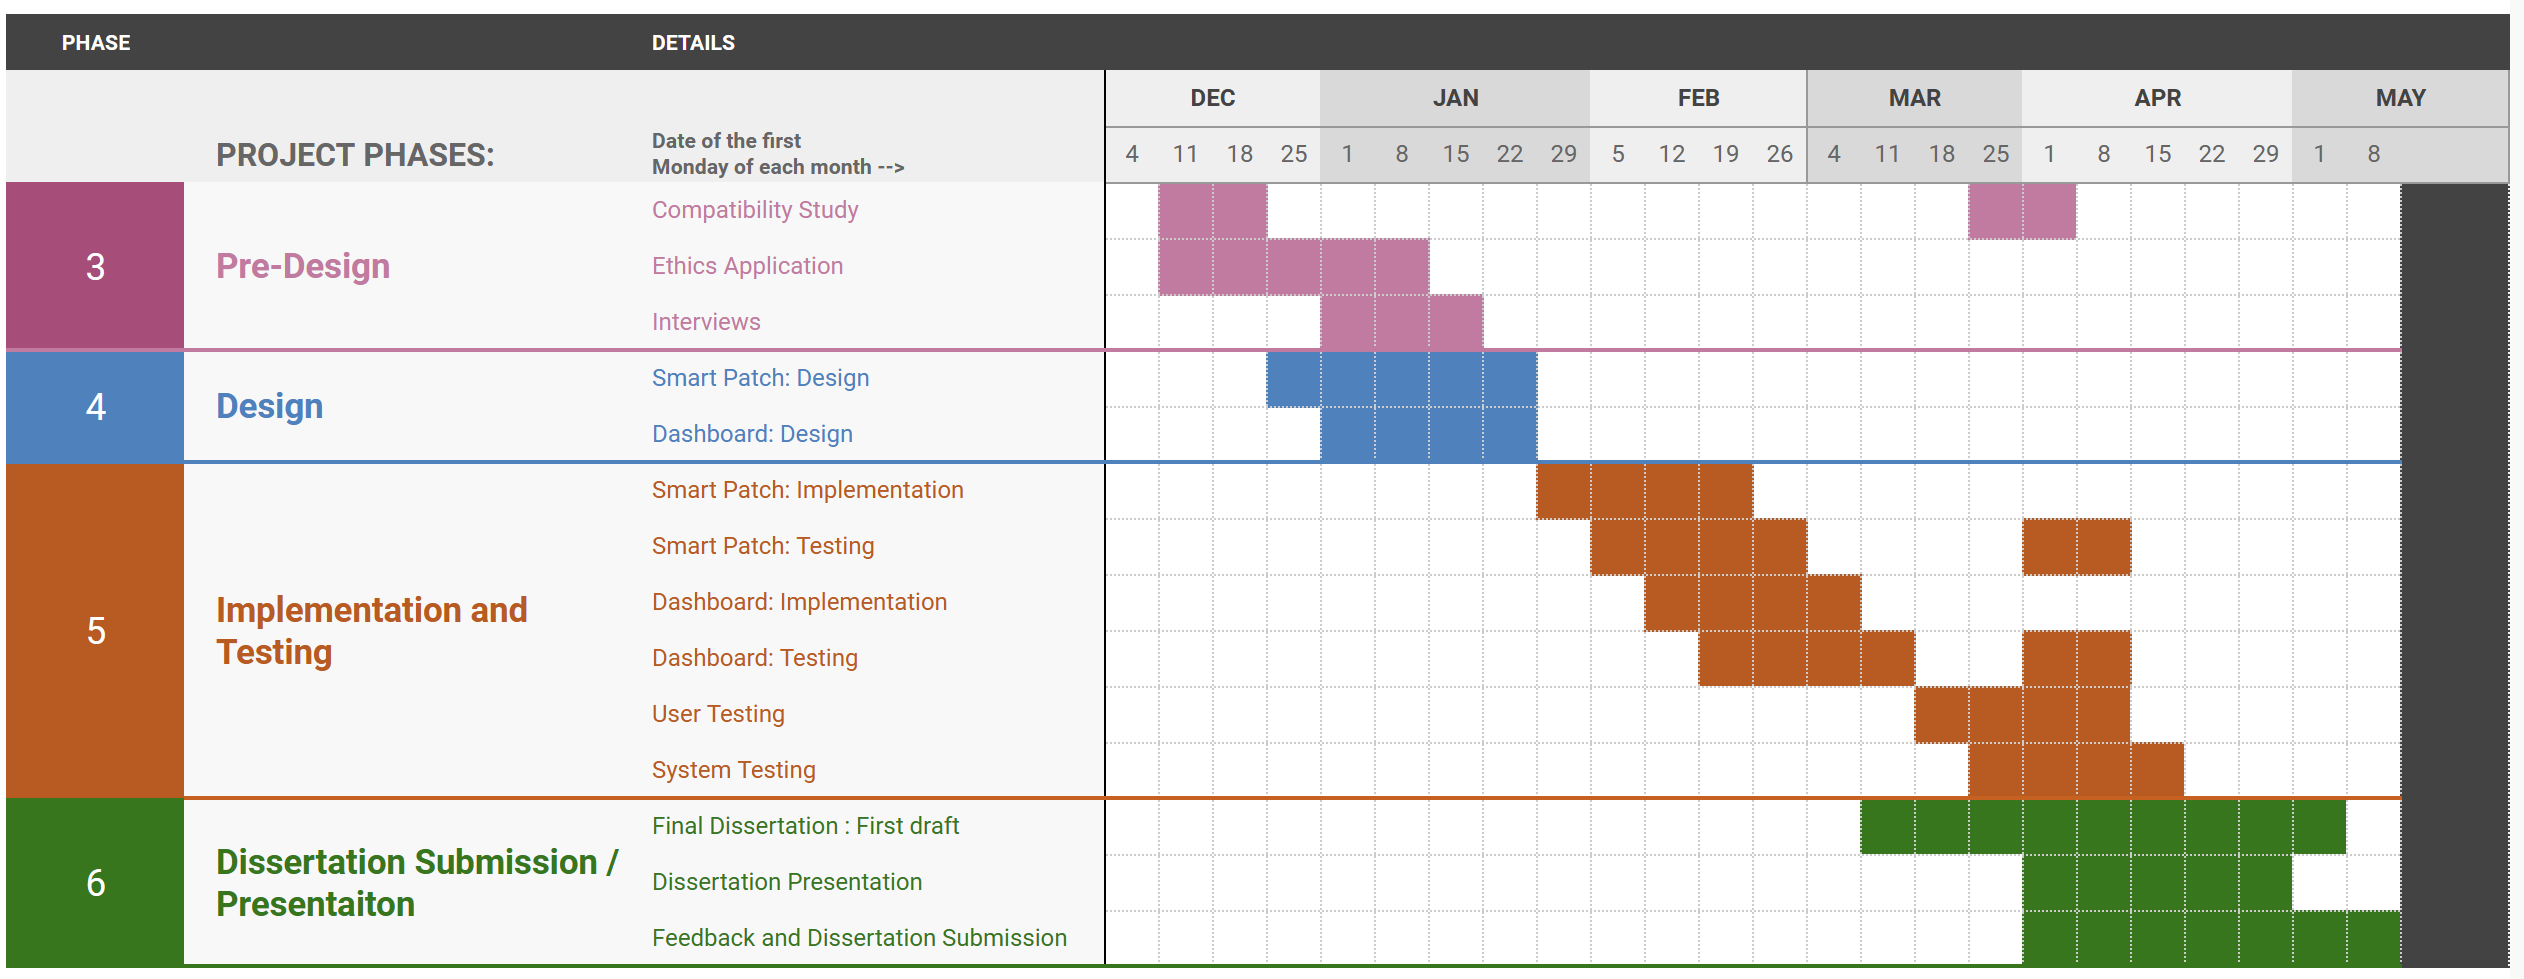
\includegraphics{images/gantt-chart.png}
%     \caption{Gantt Chart}
%     \label{fig:gantt-chart}
% \end{figure}

\section{Firmware}


The development of the Smart Patch firmware was characterized by a series of iterative improvements aimed at enhancing sensor accuracy, data handling, and user interaction. The project began with basic analog signal processing and gradually incorporated more sophisticated digital technologies and cloud-based integrations. Each iteration was driven by the dual goals of improving data reliability and enhancing user experience, while also adapting to technical challenges encountered along the way. \\

\noindent Initially, the firmware relied on analog signals to gather data from pulse sensor and LM-35 temperature sensor, which resulted in unstable and inaccurate readings. The shift to digital signal processing, and later to digital sensors like the DS18B20 for temperature sensing, marked significant advancements in data accuracy and stability. Integrating the system with cloud platforms such as Adafruit IO and external APIs like Twilio for SMS notifications brought about real-time data monitoring and interactive functionalities, further extending the capabilities of the Smart Patch. \\

\noindent The iterative development process was guided by continuous testing and feedback, which helped identify and rectify shortcomings in real-time. Challenges such as managing non-static IP addresses were addressed through architectural adjustments, notably the introduction of middleware to maintain connectivity and manageability. The final iterations focused on user management and data publishing control, allowing for more flexible and user-centric operation. \\

\noindent As of for the physical hardware - majorly the changes can be seen in from v1 to v6. Rest the hardware remained same. These can be seen in figures \ref{fig:v1-firmware} and \ref{fig:v6-firmware}.

\begin{figure}[h!]
    \centering
    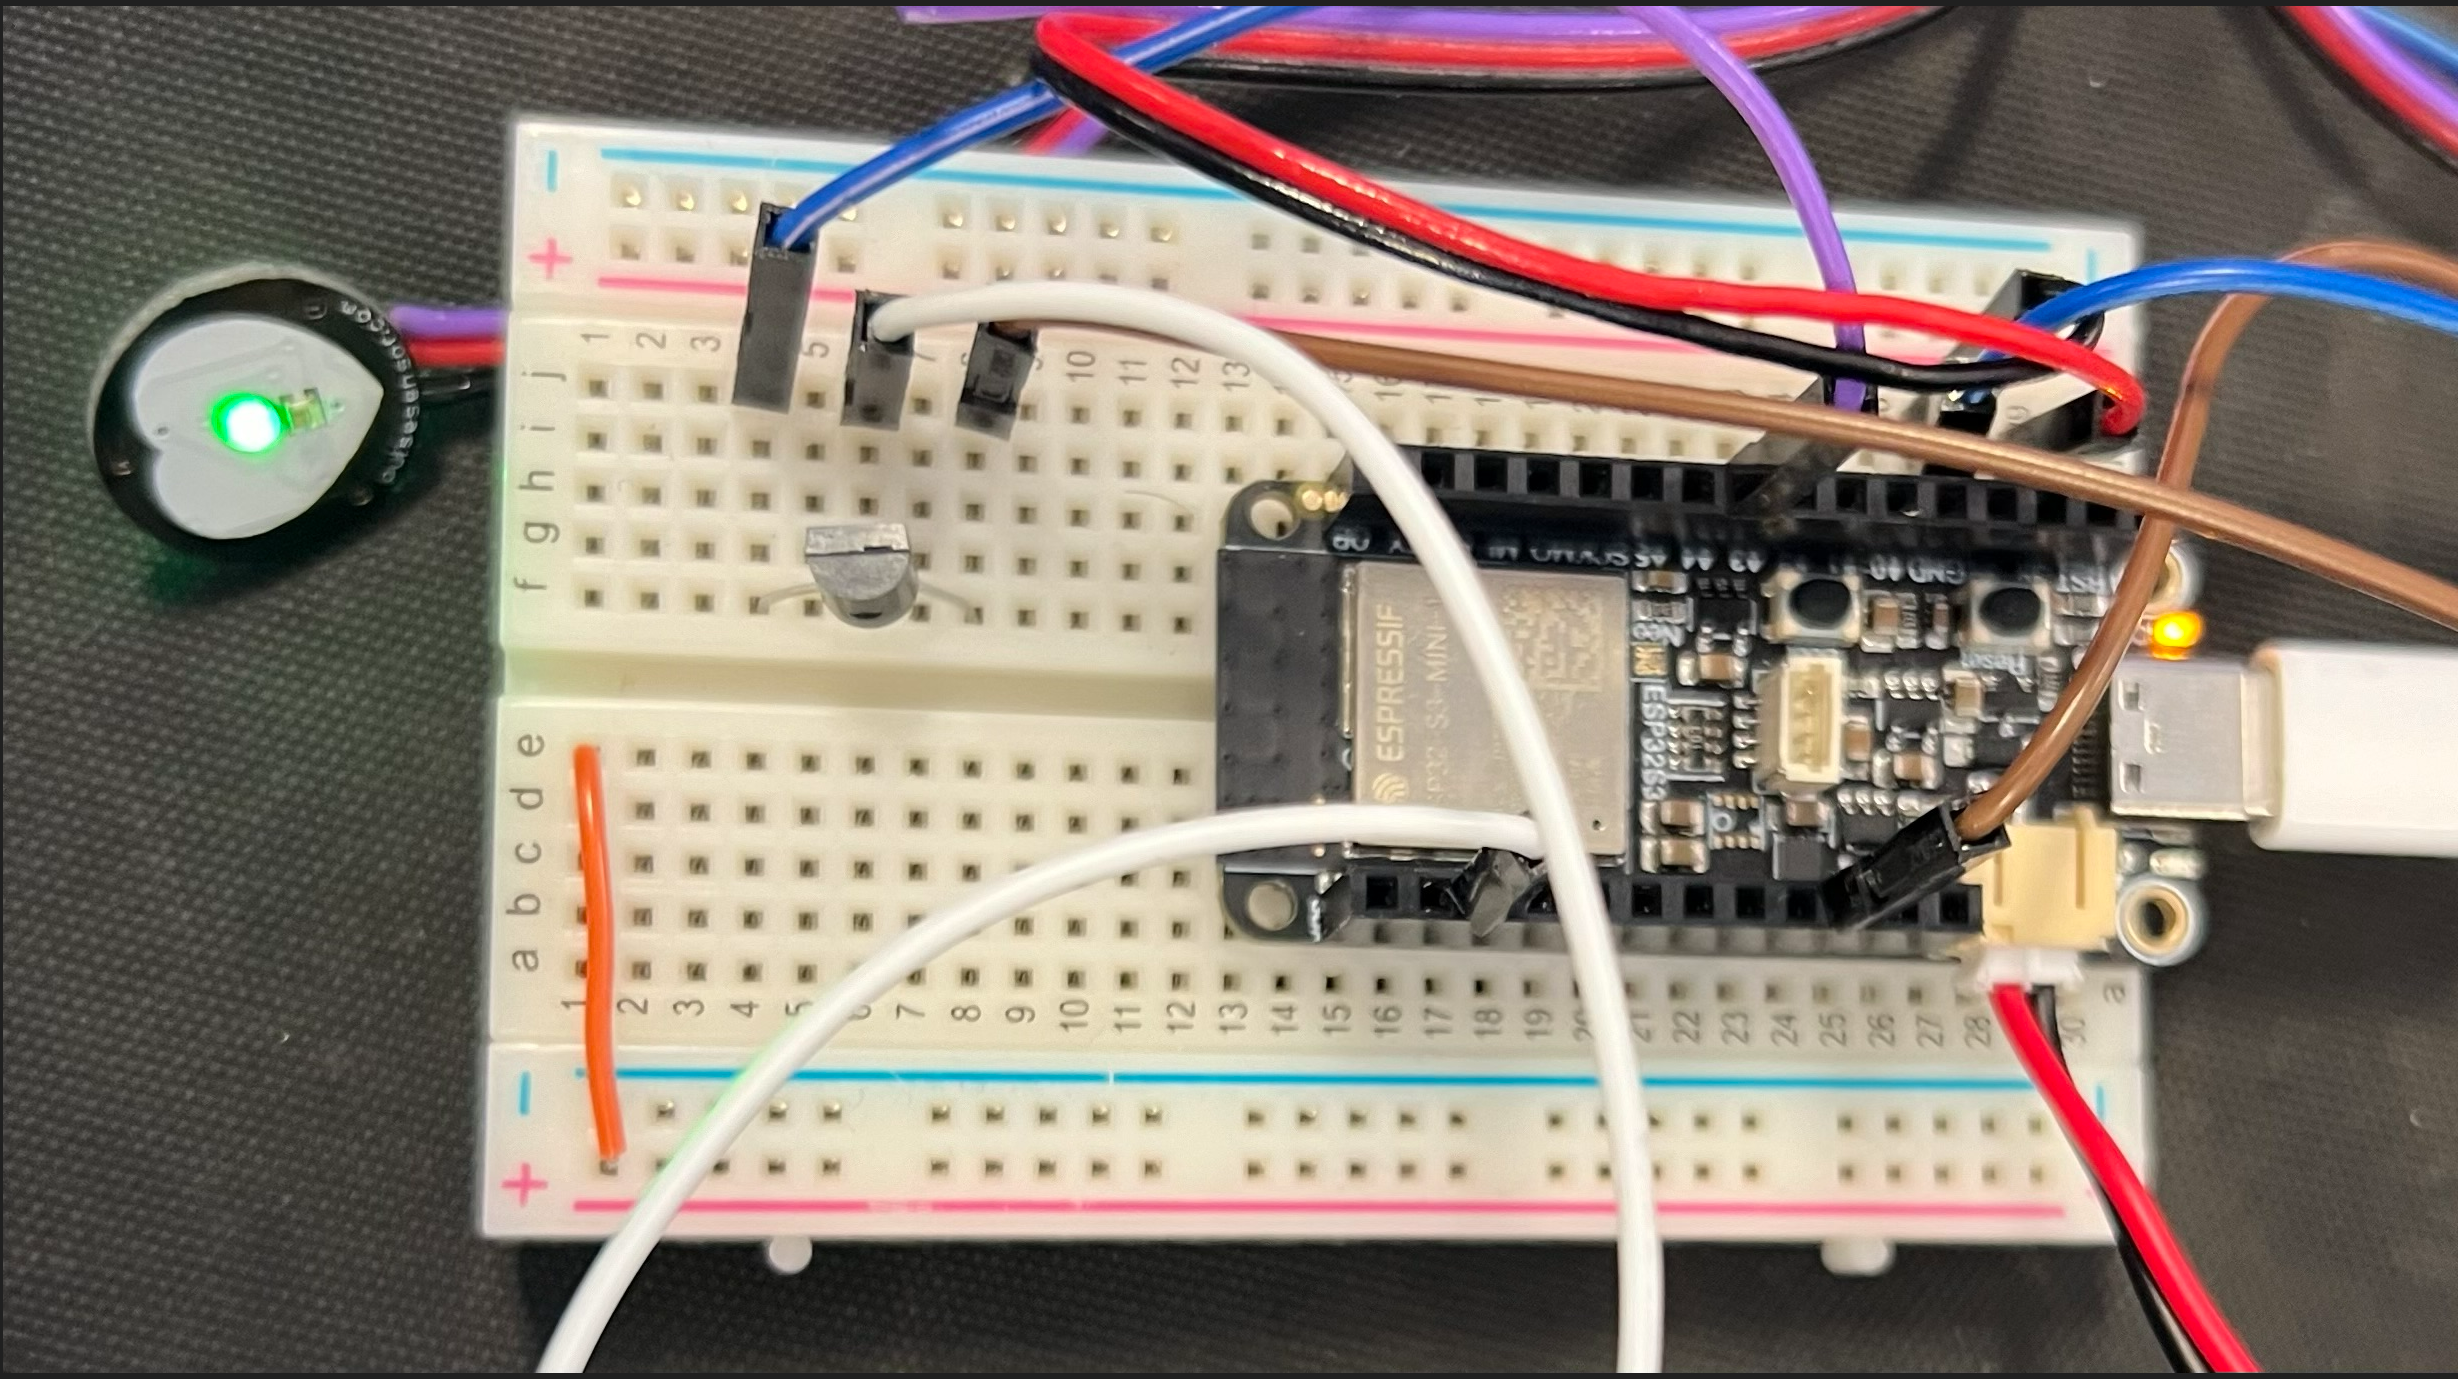
\includegraphics[width=1\linewidth]{images/v1-firmware.png}
    \caption{V1 Firmware}
    \label{fig:v1-firmware}
\end{figure}

\begin{figure}[h!]
    \centering
    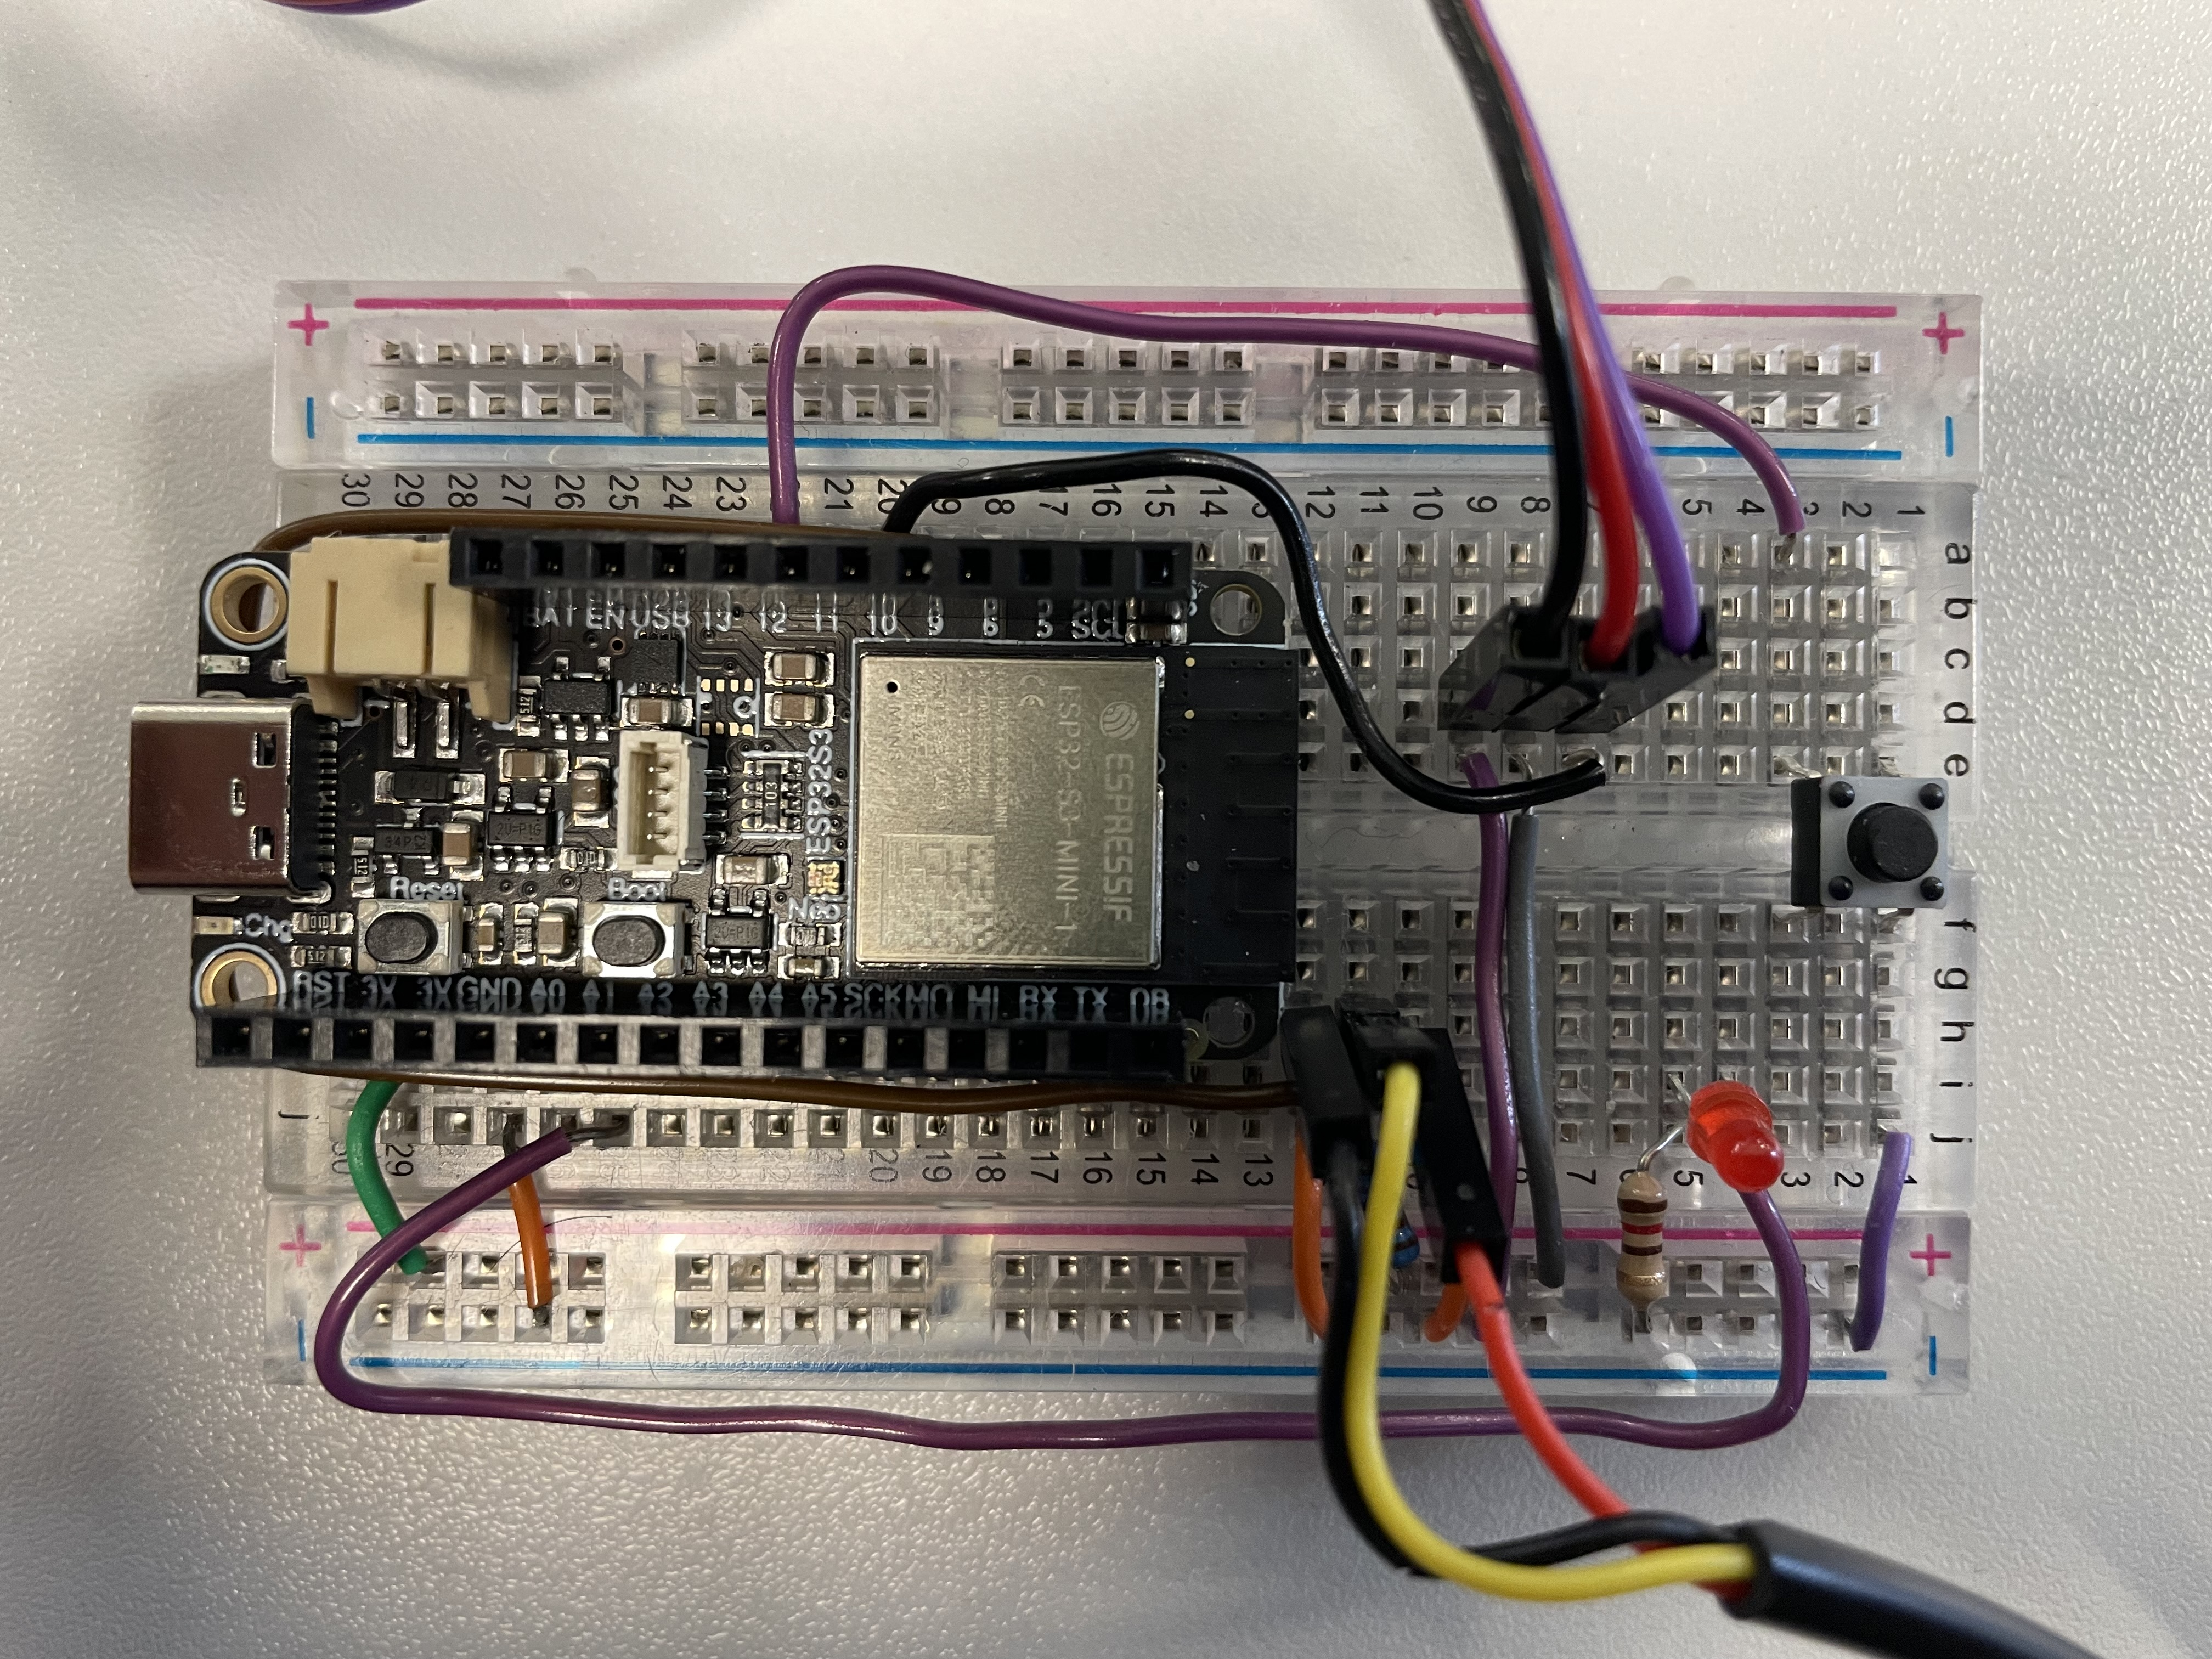
\includegraphics[width=1\linewidth]{images/v6-hardware.jpg}
    \caption{V6 Firmware}
    \label{fig:v6-firmware}
\end{figure}

\noindent Table \ref{tab:firmware_iterations} provides a summary of each iteration. \\

% \subsection{Iterative Development Journey}
% v1  - using analog signals and converting them into digital values to get data from PulseSensor and LM-35 sensor. The data received was neither accurate nor smooth.  \\
% v2 - For pulse sensor shifting from using analog signals to convert data to using libraries to get a direct digital value - LM-35 sensor's code remained same.this time to get more accurate data - collecting data of a minute removing bottom 10\% and top 10\% values to get smoother values. On testing, got to know that doing this still was not giving accurate values for temperature and as of Pulse sensor. So decided not to go forward with it. \\
% v3 - even then doing the both, was not getting a correct and smooth value from LM-35 sensor. Was advised to shift to a digital sensor - DS18B20.Tested things with it and got way more accurate and smooth data for temperature.  \\
% v4 - Connected to Wifi network, setup connected with Adafruit IO Dashboard by creating this esp as MQTT Client and publishing data on to 2 feeds - bpmFeed and temperatureFeed. These feeds were then subscribed by the dashboard. Tested whether the data is reflecting accurately and in real-time on the dashboard. Results were positive. \\
% v5 - Connected to Twilio API to send SMS when temperature crosses 35 degrees celcius. This was done statically to test the connection and how fast the SMS reaches to a person. Here the phone number is also static. Tests were positive but the messages were spamming because temperature doesn't fluctuate because if it stays above 35 it is going to be there for a while and everytime the condition is checked it will send an SMS. So added a condition that SMS will only be sent once every 30 mins. Tests were positive then.\\
% v6 - till now everything was in one file and it was becoming inefficient - divided things into separate files. Also added default values for name, phone number, and thresholds. We added a proper condition in the code comparing current values with the thresholds, only when it goes above or below the thresholds it sends an SMS. Added a switch and led to publish data only when the switch is turned on.  Created a temporary website on Flask to send data (name, phone number and thresholds) to the device - one major thing needed was the ip address and port number of the device to send/receive data. Tested to see if everything was working fine together. Results: Positive\\
% v7 - Data from the sensors were still a bit glitchy - so decided to implement Moving Average logic so that data never goes to extreme values. Gave it tolerance for each sensor so that beyond this the value should never go - if it goes skip the publishing logic. In addition to this, added an AnsyncWebServer to the device from where the temporary website could directly verify whether this device is active or not (connected to the network), to handle incoming data from the website about the user, and handle command of stop publishing when needed. Tests: Positive but a major challenge was that IP Addresses were not static. They change with changes in the network and then the data will never work out, and it would be hard for a not-so-tech-savvy person to create a static IP address for their network in the organization. So a different logic was needed to handle this - because it is not at all efficient. \\
% v8 - to handle the IP address issue, a middleware was introduced. So the idea behind it was that the middleware URL will be static and the device as soon as it gets connected to wifi will send a request to the middleware and share its IP Address which the middleware stores. Now in the user interface, organization admins don't have to know the ever-changing IP Addresses and change it every time - now they just need to remember the device's nickname and passkey which would never change. Along with this, another change in logic was made that the device should be easily switched between different users and when no users are assigned to the device, it should just not publish anything. Using that, streamlined the process by making it more about the user using it rather than about the device and making sure to get its credentials every time. To accomodate the middleware logic, had to change the code's asyncwebserver logic. Now the server's request were handled by /stop-publishing, /receive-user-details, /clear-user-details to receive data from the middleware. Along with this, it was thought that publishing data on the admin's website in addition to Adafruit IO dashboard would be quite useful to see real-time results on the same screen. This was tested well - and marked the end of Smart Patch's development. 


\begin{table}[h!]
\centering
\caption{Summary of Firmware Iterations}
\label{tab:firmware_iterations}
\begin{tabularx}{\textwidth}{|c|X|X|X|}
\hline
\textbf{Iteration} & \textbf{Description} & \textbf{Key Changes} & \textbf{Outcome} \\ \hline
v1 & Initial implementation using analog signals. & Utilized PulseSensor and LM-35 sensors with analog outputs. & Data was unstable and lacked accuracy. \\ \hline
v2 & Enhanced data handling by discarding outliers. & Implemented data smoothing by removing the top and bottom 10\% of readings; maintained analog LM-35 while shifting PulseSensor to digital. & Improved pulse data slightly; temperature readings remained unreliable. \\ \hline
v3 & Switch to digital temperature sensor. & Replaced LM-35 with DS18B20 for temperature measurements. & Achieved highly accurate and stable temperature data. \\ \hline
v4 & Integration with cloud and real-time data dashboard. & Connected to Wi-Fi; established MQTT client for Adafruit IO dashboard. & Successfully reflected real-time data on the dashboard. \\ \hline
v5 & Added SMS notifications for temperature alerts. & Integrated Twilio API to send SMS alerts when temperature exceeds 35°C; included rate-limiting. & Reduced spam with effective notification for critical temperature conditions. \\ \hline
v6 & Codebase optimization and user data management. & Refactored code into separate files; added web interface for user data input. & Enhanced efficiency and usability with better organization and user data integration. \\ \hline
v7 & Implemented data smoothing and reliability checks. & Introduced moving average logic for data smoothing and set tolerance thresholds for sensor data. & Further stabilized sensor data, but faced challenges with dynamic IP addresses. \\ \hline
v8 & Addressed connectivity issues; enhanced user management. & Implemented middleware for IP management; enhanced user-centric functionality and data privacy. & Resolved IP issues and improved system flexibility for user management and data handling. \\ \hline
\end{tabularx}
\end{table}


\noindent This section will discuss details as per the eight iteration.

\newpage
\subsection{Sensor Integration}

The integration of sensors into the firmware of the Smart Patch was a critical component of its development, enabling the device to capture real-time physiological data with high accuracy. This subsection details the integration processes for both the Pimoroni Pulse Sensor and the DS18B20 Temperature Sensor, as well as the implementation of a moving average filter to enhance sensor accuracy.

\subsubsection{Integration of Pimoroni Pulse Sensor}

The integration of the Pimoroni Pulse Sensor was implemented using the PulseSensorPlayground library to facilitate the capture of heartbeat signals. Configuration involved setting the input pin and threshold for beat detection. Below is the code used in the file \texttt{/esp/config.h}:

\begin{lstlisting}[language=C++, caption=Code for Pulse Sensor Integration]
// Pulse Sensor Setup
const int PulseWire = 10;
int Threshold = 550;
PulseSensorPlayground pulseSensor;

void setupSensors() {
    pulseSensor.analogInput(PulseWire);
    pulseSensor.setThreshold(Threshold);
    if (pulseSensor.begin()) {
        Serial.println("PulseSensor initialised!");
    }
}
\end{lstlisting}

This setup ensures that the pulse sensor is initialized correctly and ready to transmit pulse rate data to the main application.

\subsubsection{Integration of DS18B20 Temperature Sensor}

The DS18B20 Temperature Sensor, a digital sensor, was integrated using the OneWire and DallasTemperature libraries to allow for accurate temperature readings. The sensor was configured with the following initialization code (Listing~\ref{lst:temp-sensor} from the file \texttt{/esp/config.h}):

\begin{lstlisting}[language=C++, caption=Code for DS18B20 Integration, label=lst:temp-sensor]
// DS18b20 Sensor Setup
const int TempWire = 9;
OneWire oneWire(TempWire);
DallasTemperature tempSensors(&oneWire);

void setupSensors() {
    tempSensors.begin();
}
\end{lstlisting}

This configuration initializes the temperature sensor and prepares it to read temperatures in Celsius, which are then processed by the firmware.

\subsubsection{Sensor Accuracy - Moving Average}

To smooth out fluctuations in the data from both sensors and enhance accuracy, a moving average filter was implemented. This method averages the data points within a defined window to mitigate the effects of transient and noisy data. The following code (Listing~\ref{lst:moving-average} from the file \texttt{/esp/esp.ino}) illustrates the implementation of this moving average for both the pulse and temperature sensors:

\begin{lstlisting}[language=C++, caption=Implementation of Moving Average to increase sensor accuracy, label=lst:moving-average]
const int movingAverageWindowSize = 10;
float bpmSum = 0;
std::queue<int> bpmReadings;
float bpmMovingAverage = 0;
float tempSum = 0;
std::queue<float> tempReadings;
float tempMovingAverage = 0;

// Tolerance constants
const int BPM_TOLERANCE = 10; // Adjust based on testing and sensor accuracy
const float TEMP_TOLERANCE = 0.5; // Adjust based on testing and sensor accuracy

void updateMovingAverage(int bpm, float tempC) {
    // Update BPM moving average
    if (bpmReadings.size() >= movingAverageWindowSize) {
        bpmSum -= bpmReadings.front();
        bpmReadings.pop();
    }
    bpmSum += bpm;
    bpmReadings.push(bpm);
    bpmMovingAverage = bpmSum / bpmReadings.size();

    // Update Temperature moving average
    if (tempReadings.size() >= movingAverageWindowSize) {
        tempSum -= tempReadings.front();
        tempReadings.pop();
    }
    tempSum += tempC;
    tempReadings.push(tempC);
    tempMovingAverage = tempSum / tempReadings.size();
}
\end{lstlisting}

\noindent Through this implementation, both pulse and temperature readings are consistently averaged out, providing more reliable data to the system for further processing and decision-making.




\subsection{MQTT and Adafruit IO Integration}

The integration of MQTT protocol with Adafruit IO provides a robust solution for remote data monitoring and device management in the Smart Patch system. MQTT (Message Queuing Telemetry Transport) is a lightweight messaging protocol ideal for IoT applications due to its minimal bandwidth usage and effective data transmission even in unreliable networks.

\subsubsection{Configuration and Initialization}

The integration involves setting up an MQTT client with Adafruit IO as the broker. This setup utilizes the Adafruit MQTT library to establish a connection and publish data to specific feeds configured in the Adafruit IO dashboard. Below is the primary configuration used to initialize the MQTT client and data feeds:

\begin{lstlisting}[language=C++, caption={MQTT and Adafruit IO Client Configuration}]
#include "Adafruit_MQTT.h"
#include "Adafruit_MQTT_Client.h"

#define AIO_SERVER "io.adafruit.com"
#define AIO_SERVERPORT 1883
#define AIO_USERNAME "your_username"
#define AIO_KEY "your_aio_key"

// Setup the MQTT client class
Adafruit_MQTT_Client mqtt(&espClient, AIO_SERVER, AIO_SERVERPORT, AIO_USERNAME, AIO_KEY);
Adafruit_MQTT_Publish bpmFeed = Adafruit_MQTT_Publish(&mqtt, AIO_USERNAME "/feeds/BPM");
Adafruit_MQTT_Publish temperatureFeed = Adafruit_MQTT_Publish(&mqtt, AIO_USERNAME "/feeds/Temperature");
\end{lstlisting}

In this setup, the MQTT client is configured with server details and user credentials. Feeds for BPM and temperature data are defined using the username and a specific endpoint path that corresponds to each data type.


\noindent These code snippets and explanations outline the critical aspects of the MQTT and Adafruit IO integration within the Smart Patch system, demonstrating the implementation of network communication protocols to enhance IoT capabilities.

On the Adafruit IO D- the health-data dashboard looks like:

-- ADD IMAGE OF THE DASHBOARD


\subsection{Twilio Integration}

Twilio's cloud communication platform was integrated into the Smart Patch system to enable SMS notifications based on specific health data thresholds. This feature is particularly critical for immediate user notification in case of emergency health conditions. \\

\noindent The integration requires setting up authentication with Twilio's API using the account credentials and a messaging service SID, which are defined as constants. These credentials allow the device to authenticate with Twilio's servers securely and send SMS messages through the API.

\subsubsection{Sending SMS}

The function `sendSMS` constructs the request to send an SMS using HTTP POST. It constructs the URL and body dynamically using string streams and sends the request using the ESP32's HTTPClient library.

\begin{lstlisting}[language=C++, caption={Function to Send SMS via Twilio}]
bool sendSMS(const char *body) {
    std::stringstream url, urlEncodedBody;
    url << "https://api.twilio.com/2010-04-01/Accounts/" << accountNr << "/Messages";
    urlEncodedBody << "MessagingServiceSid=" << messagingServiceSid << "&To=" << to.c_str() << "&Body=" << body;

    HTTPClient http;
    http.begin(url.str().c_str());
    http.addHeader("Content-Type", "application/x-www-form-urlencoded");
    http.setAuthorization(accountNr, twilioPassword);
    int httpCode = http.POST(urlEncodedBody.str().c_str());

    http.end();
    return httpCode == 201;  // HTTP 201 indicates Created
}
\end{lstlisting}

\subsubsection{Threshold Alerts and SMS Notification Timing}

The system sends an SMS when temperature or BPM readings cross predefined thresholds. An important feature is the timing control, ensuring SMS alerts are sent no more than once every 30 minutes, regardless of sensor reading fluctuations.

\begin{lstlisting}[language=C++, caption={Conditional SMS Notifications Based on Thresholds}]
if (tempC > temp_upper_threshold || tempC < temp_lower_threshold || (bpm > bpm_upper_threshold && bpm > 0) || (bpm < bpm_lower_threshold && bpm > 0)) {
    unsigned long currentMillis = millis();  // Get current time in milliseconds
    // Check if at least 30 minutes have passed since the last SMS
    if (currentMillis - lastSMSTime >= 1800000) {
        char smsString[240]; 
        sprintf(smsString, "%s's Health Alert: Body Temperature has crossed %.2f°C and current BPM is %d.", name, tempC, bpm);
        if (sendSMS(smsString)) {
            lastSMSTime = currentMillis;  // Update the last SMS timestamp
            Serial.println("SMS sent successfully");
        } else {
            Serial.println("Failed to send SMS");
        }
    }
}
\end{lstlisting}

These segments of code highlight how the Twilio API is utilized for real-time health monitoring and alerting via SMS, enhancing the Smart Patch's capability to respond to critical health events efficiently.









\section{Middleware}
The Middleware component of the VitalMonitor system plays a crucial role as the intermediary layer that facilitates data communication and integration between the Smart Patch, the Dashboard, and the cloud-based database. Developed using the Flask framework, this Middleware is pivotal in managing the data flow within the system, ensuring that interactions are seamless and efficient.

\subsection{Connection with Google Cloud}
Key configurations of the middleware included establishing a connection to a Google Cloud MySQL instance via Unix sockets, ensuring secure and reliable database interactions. The use of environment variables (.env file) for sensitive information like database credentials was implemented.

\begin{lstlisting}[language=python, caption={Connection to Google Cloud MySQL using unix socket} label={lst:unix-socket}]
def connect_unix_socket() -> sqlalchemy.engine.base.Engine:
    """Initializes a Unix socket connection pool for a Cloud SQL instance of MySQL."""

    db_user = os.environ["DB_USER"]  # e.g. 'my-database-user'
    db_pass = os.environ["DB_PASS"]  # e.g. 'my-database-password'
    db_name = os.environ["DB_NAME"]  # e.g. 'my-database'
    unix_socket_path = os.environ[
        "INSTANCE_UNIX_SOCKET"
    ]  # e.g. '/cloudsql/project:region:instance'

    pool = sqlalchemy.create_engine(
        # Equivalent URL:
        # mysql+pymysql://<db_user>:<db_pass>@/<db_name>?unix_socket=<socket_path>/<cloud_sql_instance_name>
        sqlalchemy.engine.url.URL.create(
            drivername="mysql+pymysql",
            username=db_user,
            password=db_pass,
            database=db_name,
            host='34.147.167.209',
            query={
                "ssl_ca": "./permissions/server-ca.pem",
                "ssl_cert": "./permissions/client-cert.pem",
                "ssl_key": "./permissions/client-key.pem",
                "ssl_verify_cert": "false"
            },
        ),
    )

    return pool
\end{lstlisting}


\subsection{Database Integration}
The Middleware's database schema was designed to support complex data structures, involving multiple tables such as \textit{Organizations}, \textit{Users}, \textit{Devices}, and \textit{DeviceData}, each serving distinct data storage and retrieval functionalities. SQLAlchemy ORM was utilized for database operations, simplifying CRUD operations and enhancing the maintainability of the code. Flask-Migrate was integrated for handling database migrations, which assists in evolving the database schema over time without losing data.


\subsubsection{Security and Performance}
Security in data handling is paramount, especially given the sensitive nature of the stored health data. The \textit{Organization} model employs the Flask-Bcrypt library for secure password handling:

\begin{lstlisting}[language=python, caption={Secure Password Handling in Organization Model}]
from flask_bcrypt import Bcrypt

bcrypt = Bcrypt()

class Organization(db.Model):
    __tablename__ = 'organizations'
    password_hash = db.Column(db.String(255), nullable=False)

    def set_password(self, password):
        self.password_hash = bcrypt.generate_password_hash(password).decode('utf-8')

    def check_password(self, password):
        return bcrypt.check_password_hash(self.password_hash, password)
\end{lstlisting}

The connection between the middleware and Google Cloud is more secure by using permission files (used in Listing \ref{lst:unix-socket}) which can only be generated once from the cloud. Without these permissions files, middleware won't get connected to the cloud.

\subsection{API Integration}

API endpoints were carefully crafted to support essential operations such as user and device registration, login processes, and data transmission between devices and the Dashboard. These endpoints handle data validation, session management, and error responses effectively, ensuring a seamless user experience and robust data handling.

\subsubsection{User and Organization Management}

The API endpoints for registering organizations and users are fundamental for setting up and securing access to the system. They ensure that only authorized entities can register and manage devices and users. Below are examples of these key functionalities:

\begin{lstlisting}[language=python, caption={API Endpoint for Organization Registration}]
@app.route('/register', methods=['POST'])
def register_organization():
    data = request.json
    name = data.get('name')
    password = data.get('password')
    if not name or not password:
        return jsonify({"error": "Name and password are required"}), 400
    if Organization.query.filter_by(name=name).first():
        return jsonify({"error": "Organization already exists"}), 400
    new_organization = Organization(name=name)
    new_organization.set_password(password)
    db.session.add(new_organization)
    try:
        db.session.commit()
    except Exception as e:
        db.session.rollback()
        return jsonify({"error": str(e)}), 500
    return jsonify({"success": "Organization registered successfully", "organization_id": new_organization.id, "organization_name": name}), 201
\end{lstlisting}

\noindent This endpoint performs critical checks such as validation of input fields and checks against existing records, ensuring data integrity and preventing duplicates in the system.

\subsubsection{Device Management}

Device management is crucial for tracking and updating the status and configuration of devices connected to the system. The API allows for device addition, updates, and assignment to users or organizations, as shown in the following example:

\begin{lstlisting}[language=python, caption={API Endpoint for Adding or Updating a Device}]
@app.route('/add-new-device', methods=['POST'])
def add_or_update_device():
    data = request.json
    mac_address = data.get('mac_address')
    ip_address = data.get('ip_address')
    passkey = data.get('passkey')
    nickname = data.get('nickname')
    device = Device.query.filter_by(mac_address=mac_address).first()
    if device:
        device.ip_address = ip_address
    else:
        device = Device(mac_address=mac_address, ip_address=ip_address, nickname=nickname, passkey=passkey)
        db.session.add(device)
    try:
        db.session.commit()
        return jsonify({"success": "Device added or updated successfully", "device_id": device.id}), 201
    except Exception as e:
        db.session.rollback()
        return jsonify({"error": str(e)}), 500
\end{lstlisting}

\noindent This endpoint not only facilitates the registration of new devices but also handles updates to existing ones, demonstrating the dynamic nature of device management within the system.

\subsubsection{Real-Time Data Interaction}

For real-time interaction, APIs facilitate the immediate relay of data between the devices and the system. This includes sending updated configuration details to the devices or receiving real-time data for display on the dashboard.

\begin{lstlisting}[language=python, caption={API Endpoint for Real-Time Data Streaming}]
@app.route('/get-device-data/<int:device_id>', methods=['GET'])
def get_device_data(device_id):
    def generate():
        with app.app_context():
            while True:
                latest_data = DeviceData.query.filter_by(device_id=device_id).order_by(DeviceData.timestamp.desc()).first()
                yield f"data:{json.dumps({'bpm': latest_data.bpm, 'temperature': latest_data.temperature})}\n\n"
                time.sleep(5)  # Adjust as necessary for your application's needs
    return Response(generate(), content_type='text/event-stream', headers={'Cache-Control': 'no-cache'})
\end{lstlisting}

\noindent This streaming API is essential for maintaining a live dashboard that reflects the most current data from connected devices.

\noindent These API integrations are pivotal in ensuring that the Middleware efficiently handles all communications within the VitalMonitor system, thus supporting robust, scalable, and secure operations.


\section{Web Dashboard}
The implementation phase of the Web Dashboard for the VitalMonitor system was guided by a commitment to reliability, security, and enhancing user efficiency. Leveraging a streamlined technology stack composed of Flask, HTML, CSS, and JavaScript, the development went beyond merely meeting functional requirements. It also focused on delivering an engaging and effective user experience for organization administrators. Most of the development is very straightforward and didn't involve much complexities unlike for Smart Patch and Middleware. Some important implementations of certain components of the website are discussed below.

\subsection{Session Management using custom decorators}

As per the design discussed in the last chapter, Custom Decorators were used for session management. Custom Decorators are nothing but a function that adds functionality to another function or method without modifying its structure. This is particularly useful in web development for handling tasks like authentication and authorization. In this case provided in Listing \ref{Session Management}, \textit{@login\_required} decorator, it acts as a gatekeeper for routes that require user authentication. \\ 

When applied, such as before the \textit{add\_device\_page()} function, the \textit{login\_required} decorator checks whether the \textit{organization\_id} exists in the session. This \textit{organization\_id} is crucial as it signifies that the admin representing an organization is currently logged in. If the check fails (i.e., if \textit{organization\_id} is not found), it redirects the admin to the login page. This prevents unauthorized users or admins from accessing routes that are meant to be secured, thereby protecting sensitive actions like adding devices.

\begin{lstlisting}[language=python, caption=Custom Decorator - login\_required, label=Session Management]
def login_required(f):
    @wraps(f)
    def decorated_function(*args, **kwargs):
        if 'organization_id' not in session:
            return redirect(url_for('register_login_page'))
        return f(*args, **kwargs)
    return decorated_function

@app.route('/add-device-page')
    @login_required
    def add_device_page():
        organization_name = session.get('organization_name')
        return render_template('add_device.html', organization_name=organization_name)
\end{lstlisting}


\subsection{Real-time Data}

The real-time data fetching mechanism is used for user pages. Figure \ref{fig:user-page-real-time-fetching-code} demonstrated in the JavaScript code utilizes Server-Sent Events (SSE) to establish a continuous stream from a server to the web browser. Specifically, the function \textit{startLiveDataStream(deviceId)} initiates the connection using the EventSource API, which connects to a specified URL that corresponds to the device ID. Once connected, the server streams data in real-time, sending updates that are automatically received by the client-side JavaScript. Additionally, the function implements robust error handling and auto-reconnect features. If the connection fails or the page becomes invisible, the connection is closed, and attempts to reconnect are made automatically, ensuring continuous data delivery without manual refresh.

\begin{figure}[h!]
    \centering
    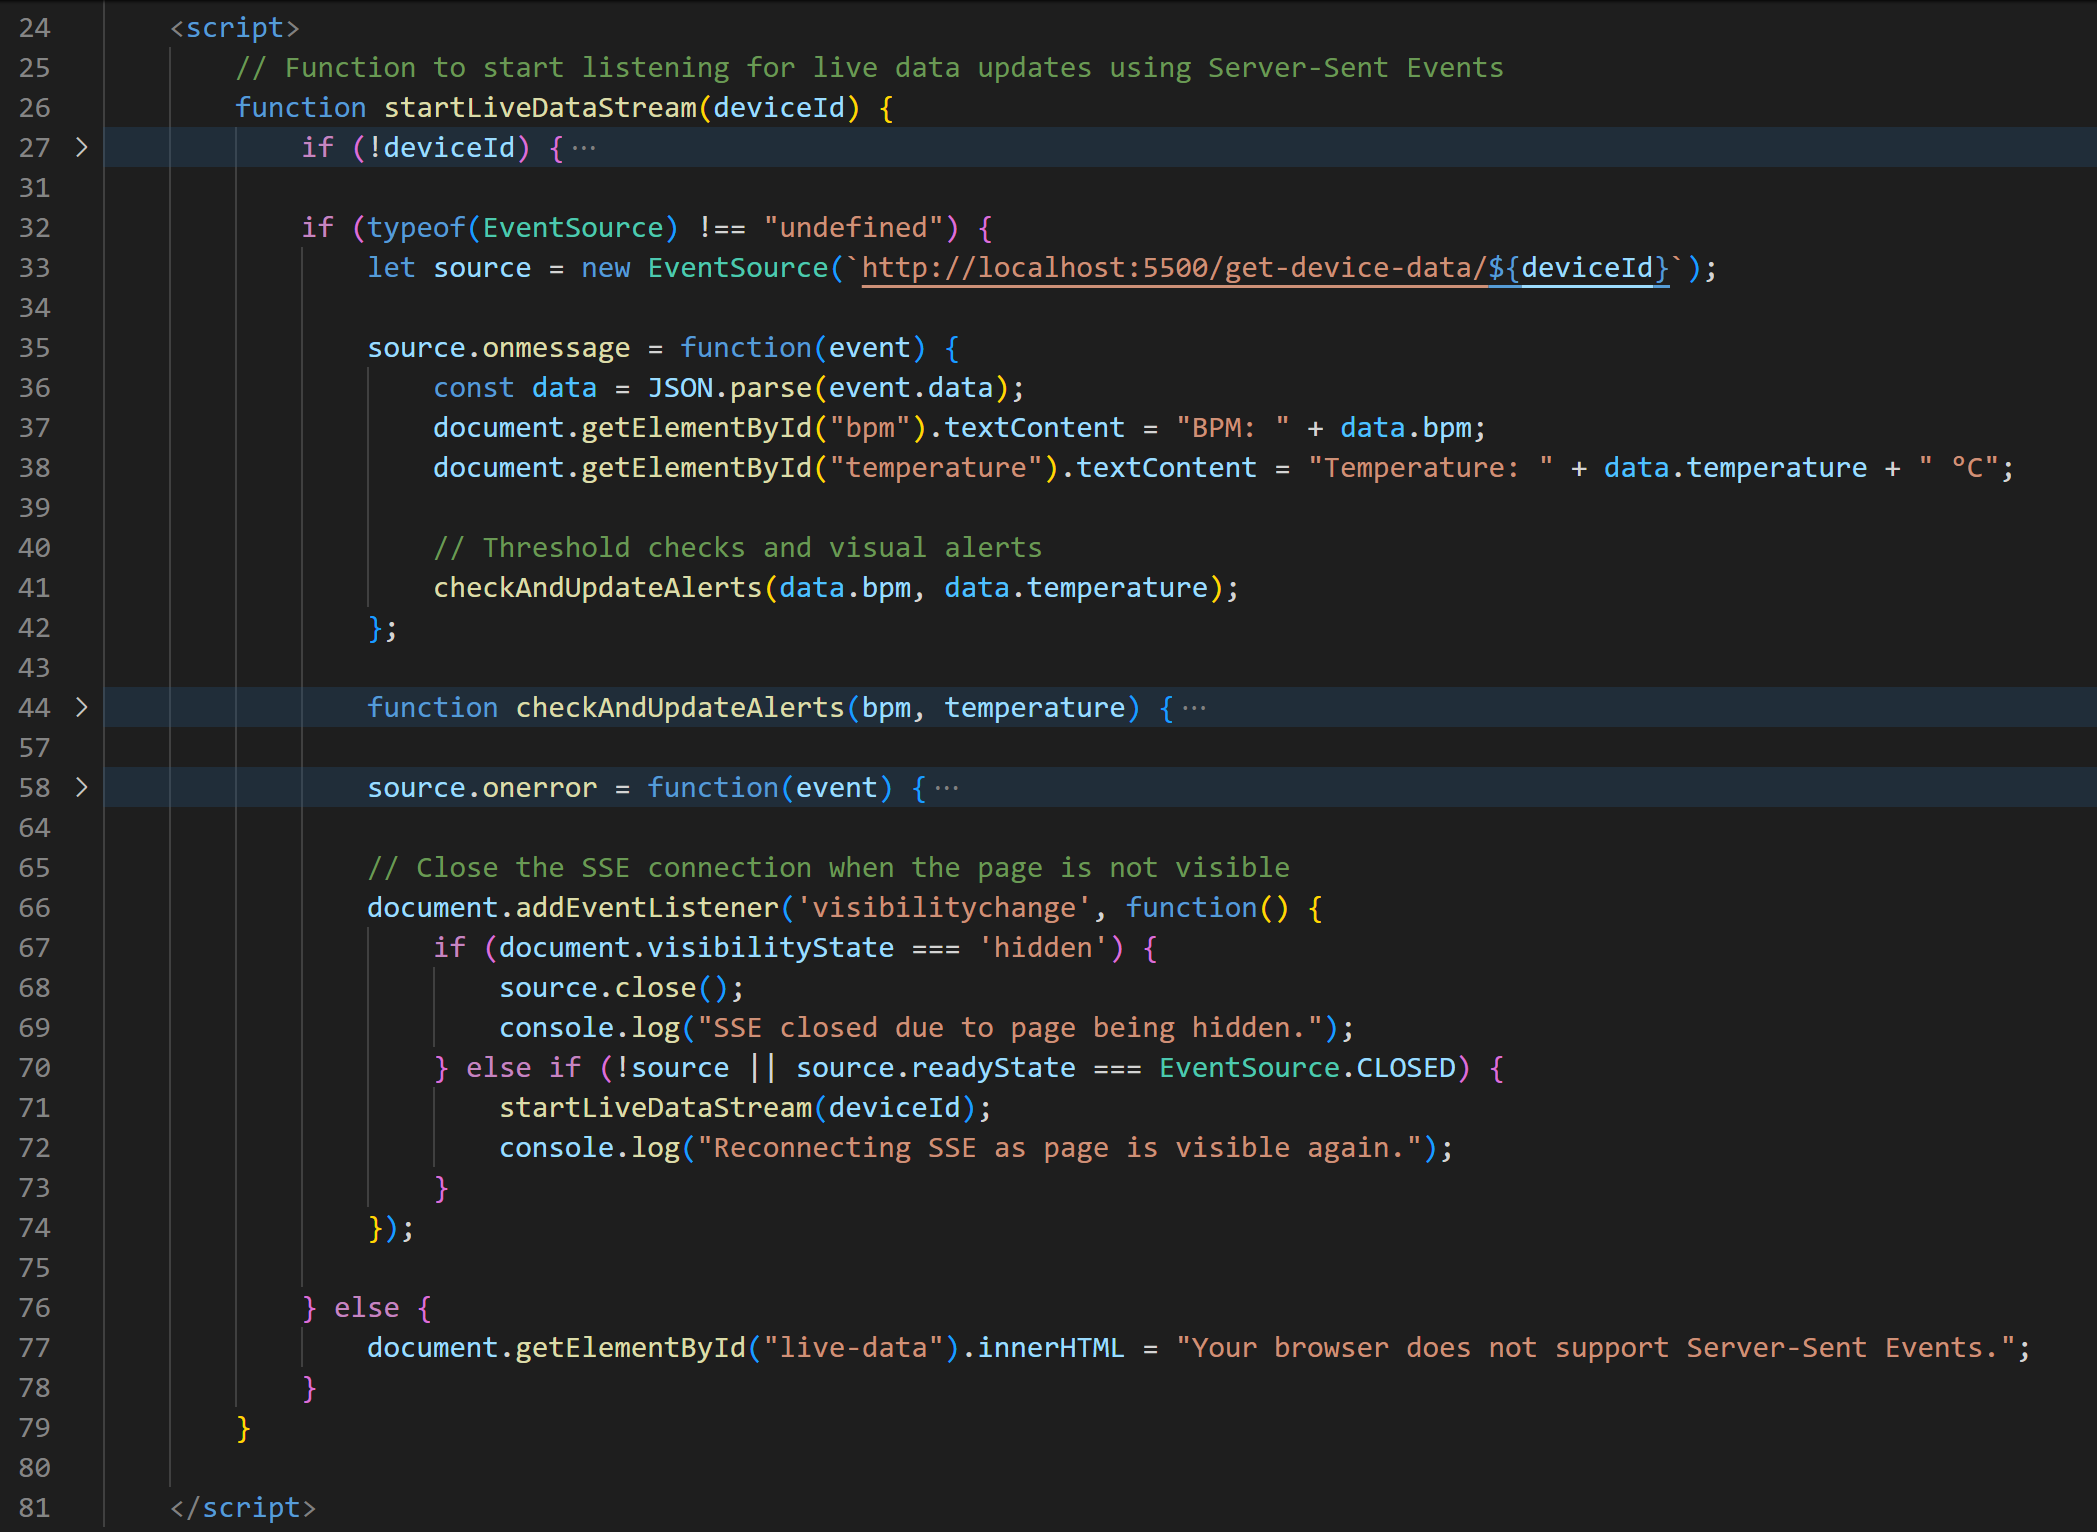
\includegraphics[width=1\linewidth]{images/user-page-real-time-fetching-code.png}
    \caption{Fetching User Health Data in real-time.}
    \label{fig:user-page-real-time-fetching-code}
\end{figure}

\subsection{User Interface and Interaction}
The design of the dashboard prioritizes ease of use and a minimalistic approach as seen in Figures \ref{fig:login-page} - \ref{fig:about-page}. Two major things that were taken care of while implementing the UI were:

\begin{itemize}

    \item \textbf{User Navigation:}
     The dashboard layout emphasizes navigational clarity, allowing admins to smoothly transition between viewing all users, managing individual profiles, and device settings without complex navigation steps.
    
    \item \textbf{Actionable Insights:}
     Interactive elements such as buttons and links are strategically placed to facilitate the easy completion of administrative tasks, such as adding or updating user information, managing devices, and monitoring health vitals.

\end{itemize}

\begin{figure}[h!]
    \centering
    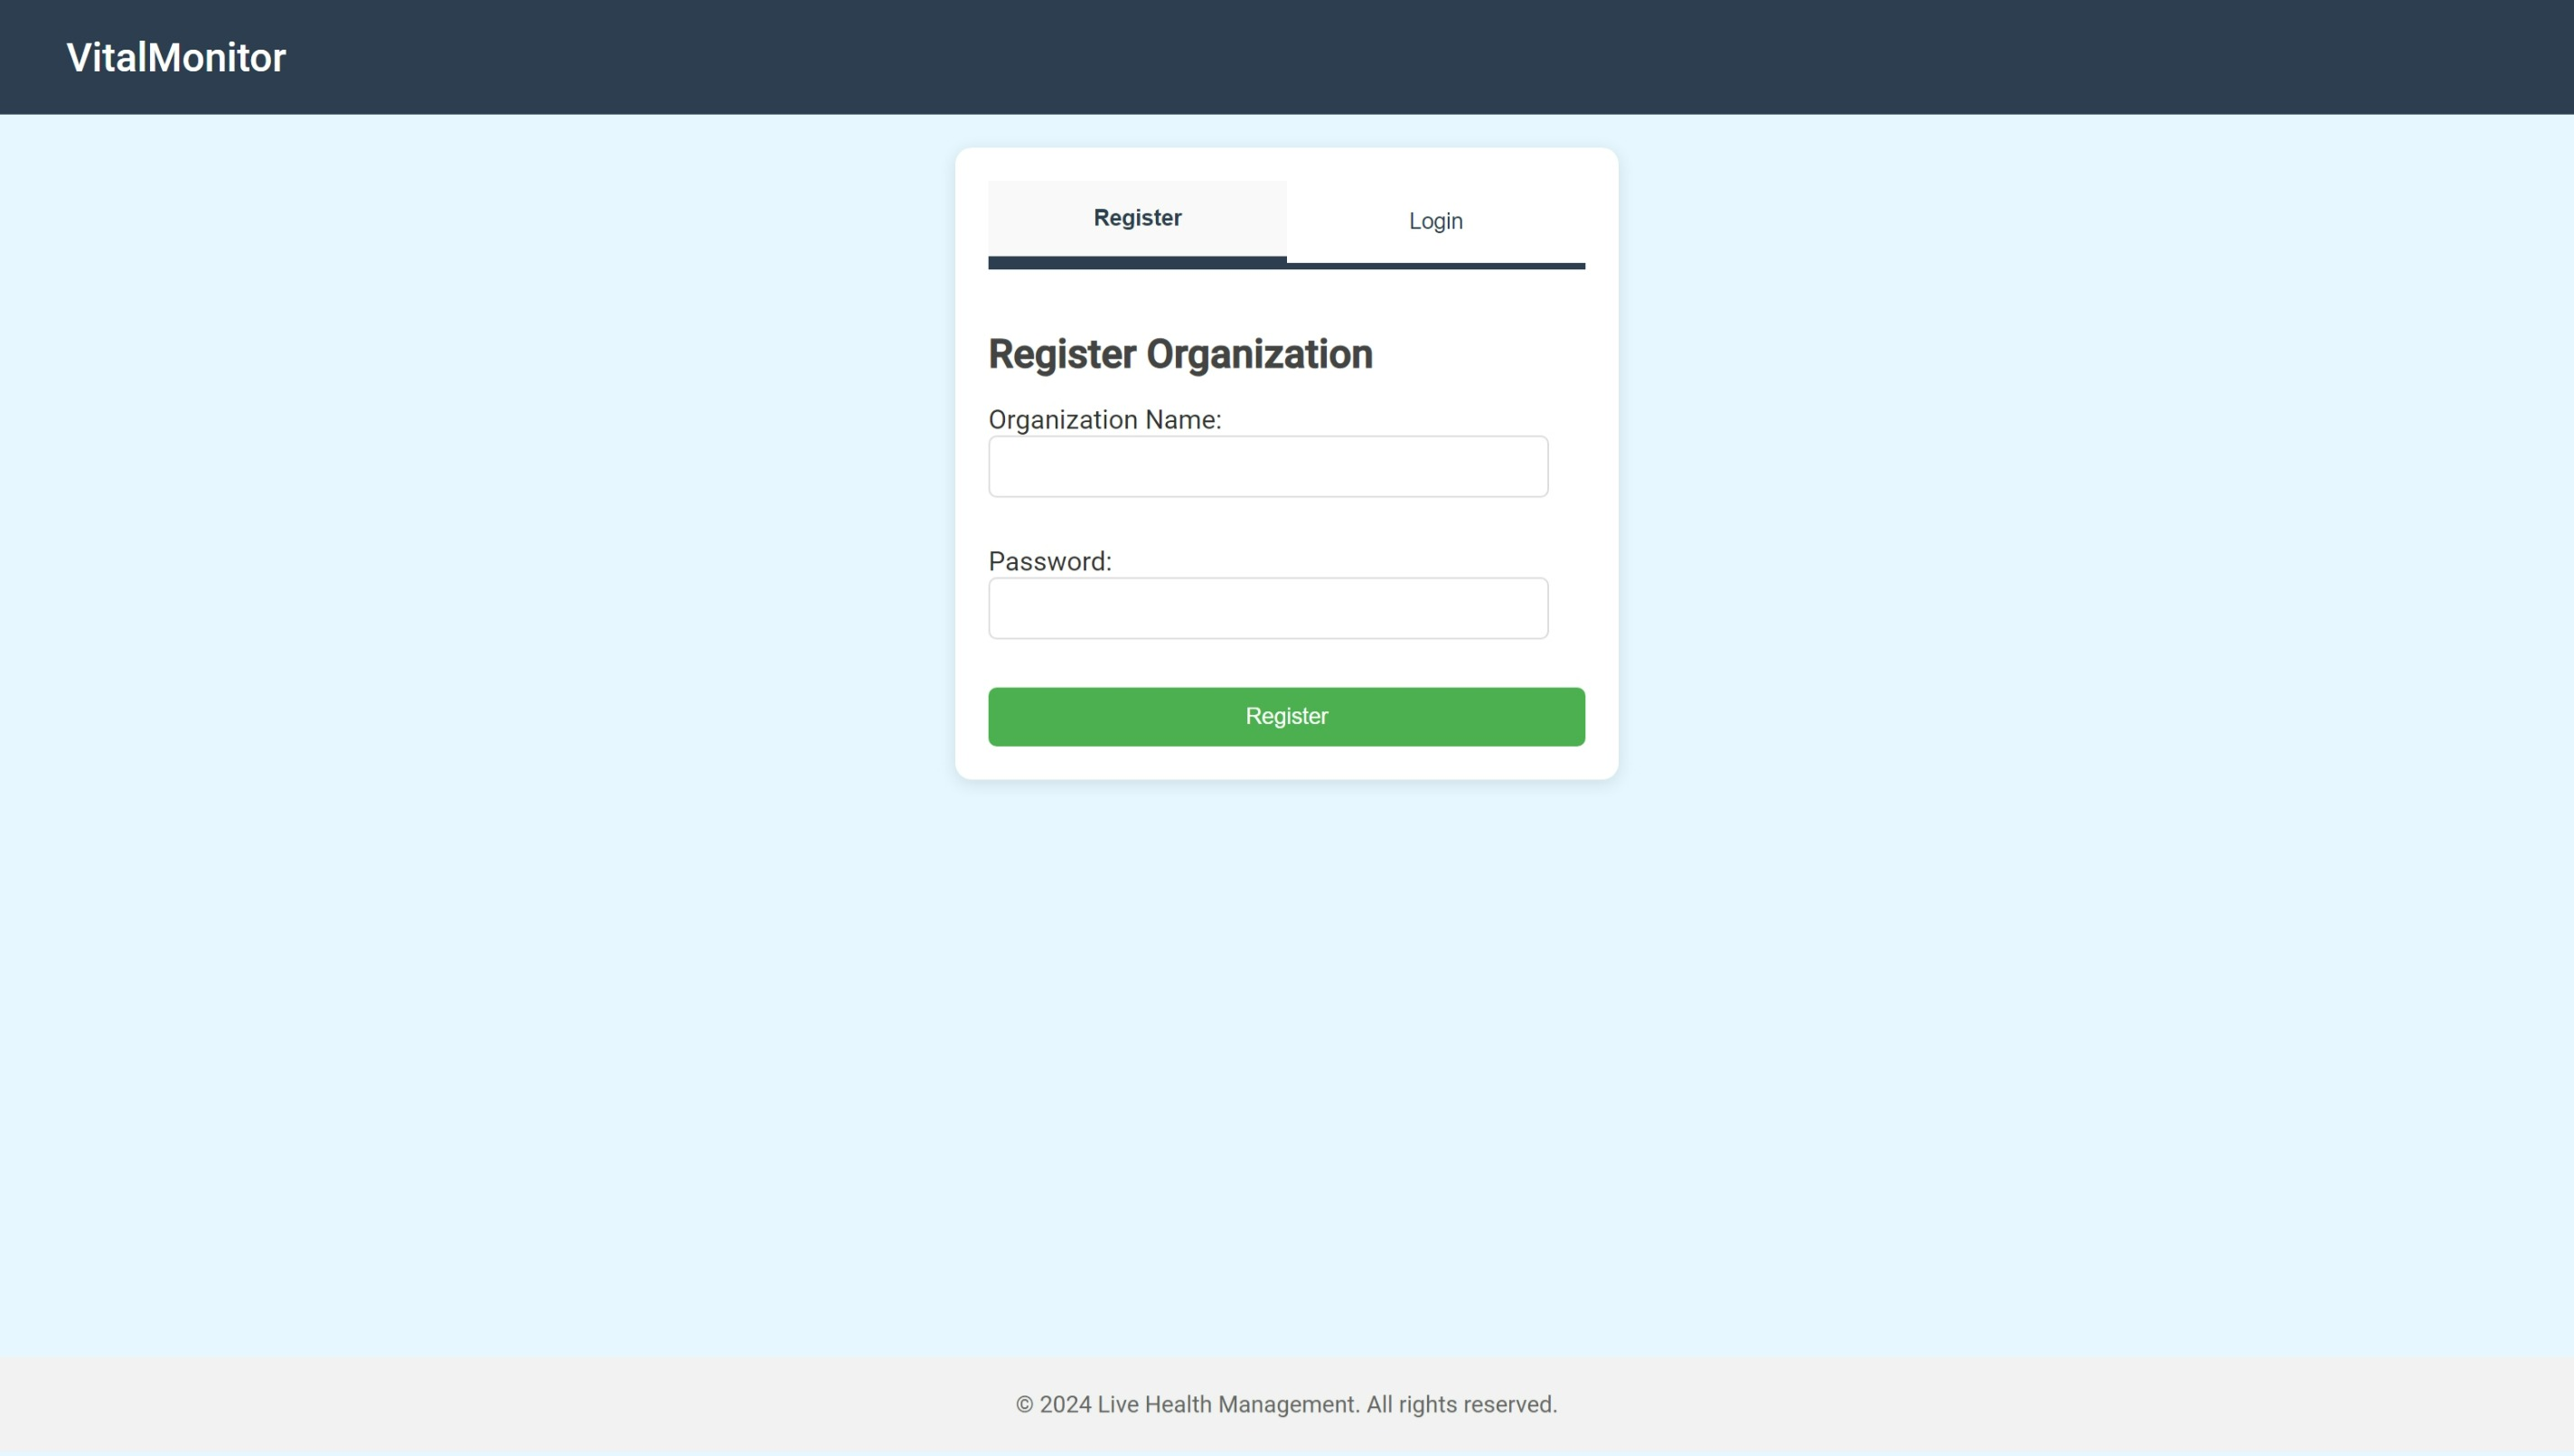
\includegraphics[width=1\linewidth]{images/dashboard-6.jpeg}
    \caption{Login and Register Page (landing page)}
    \label{fig:login-page}
\end{figure}

\begin{figure}[h!]
    \centering
    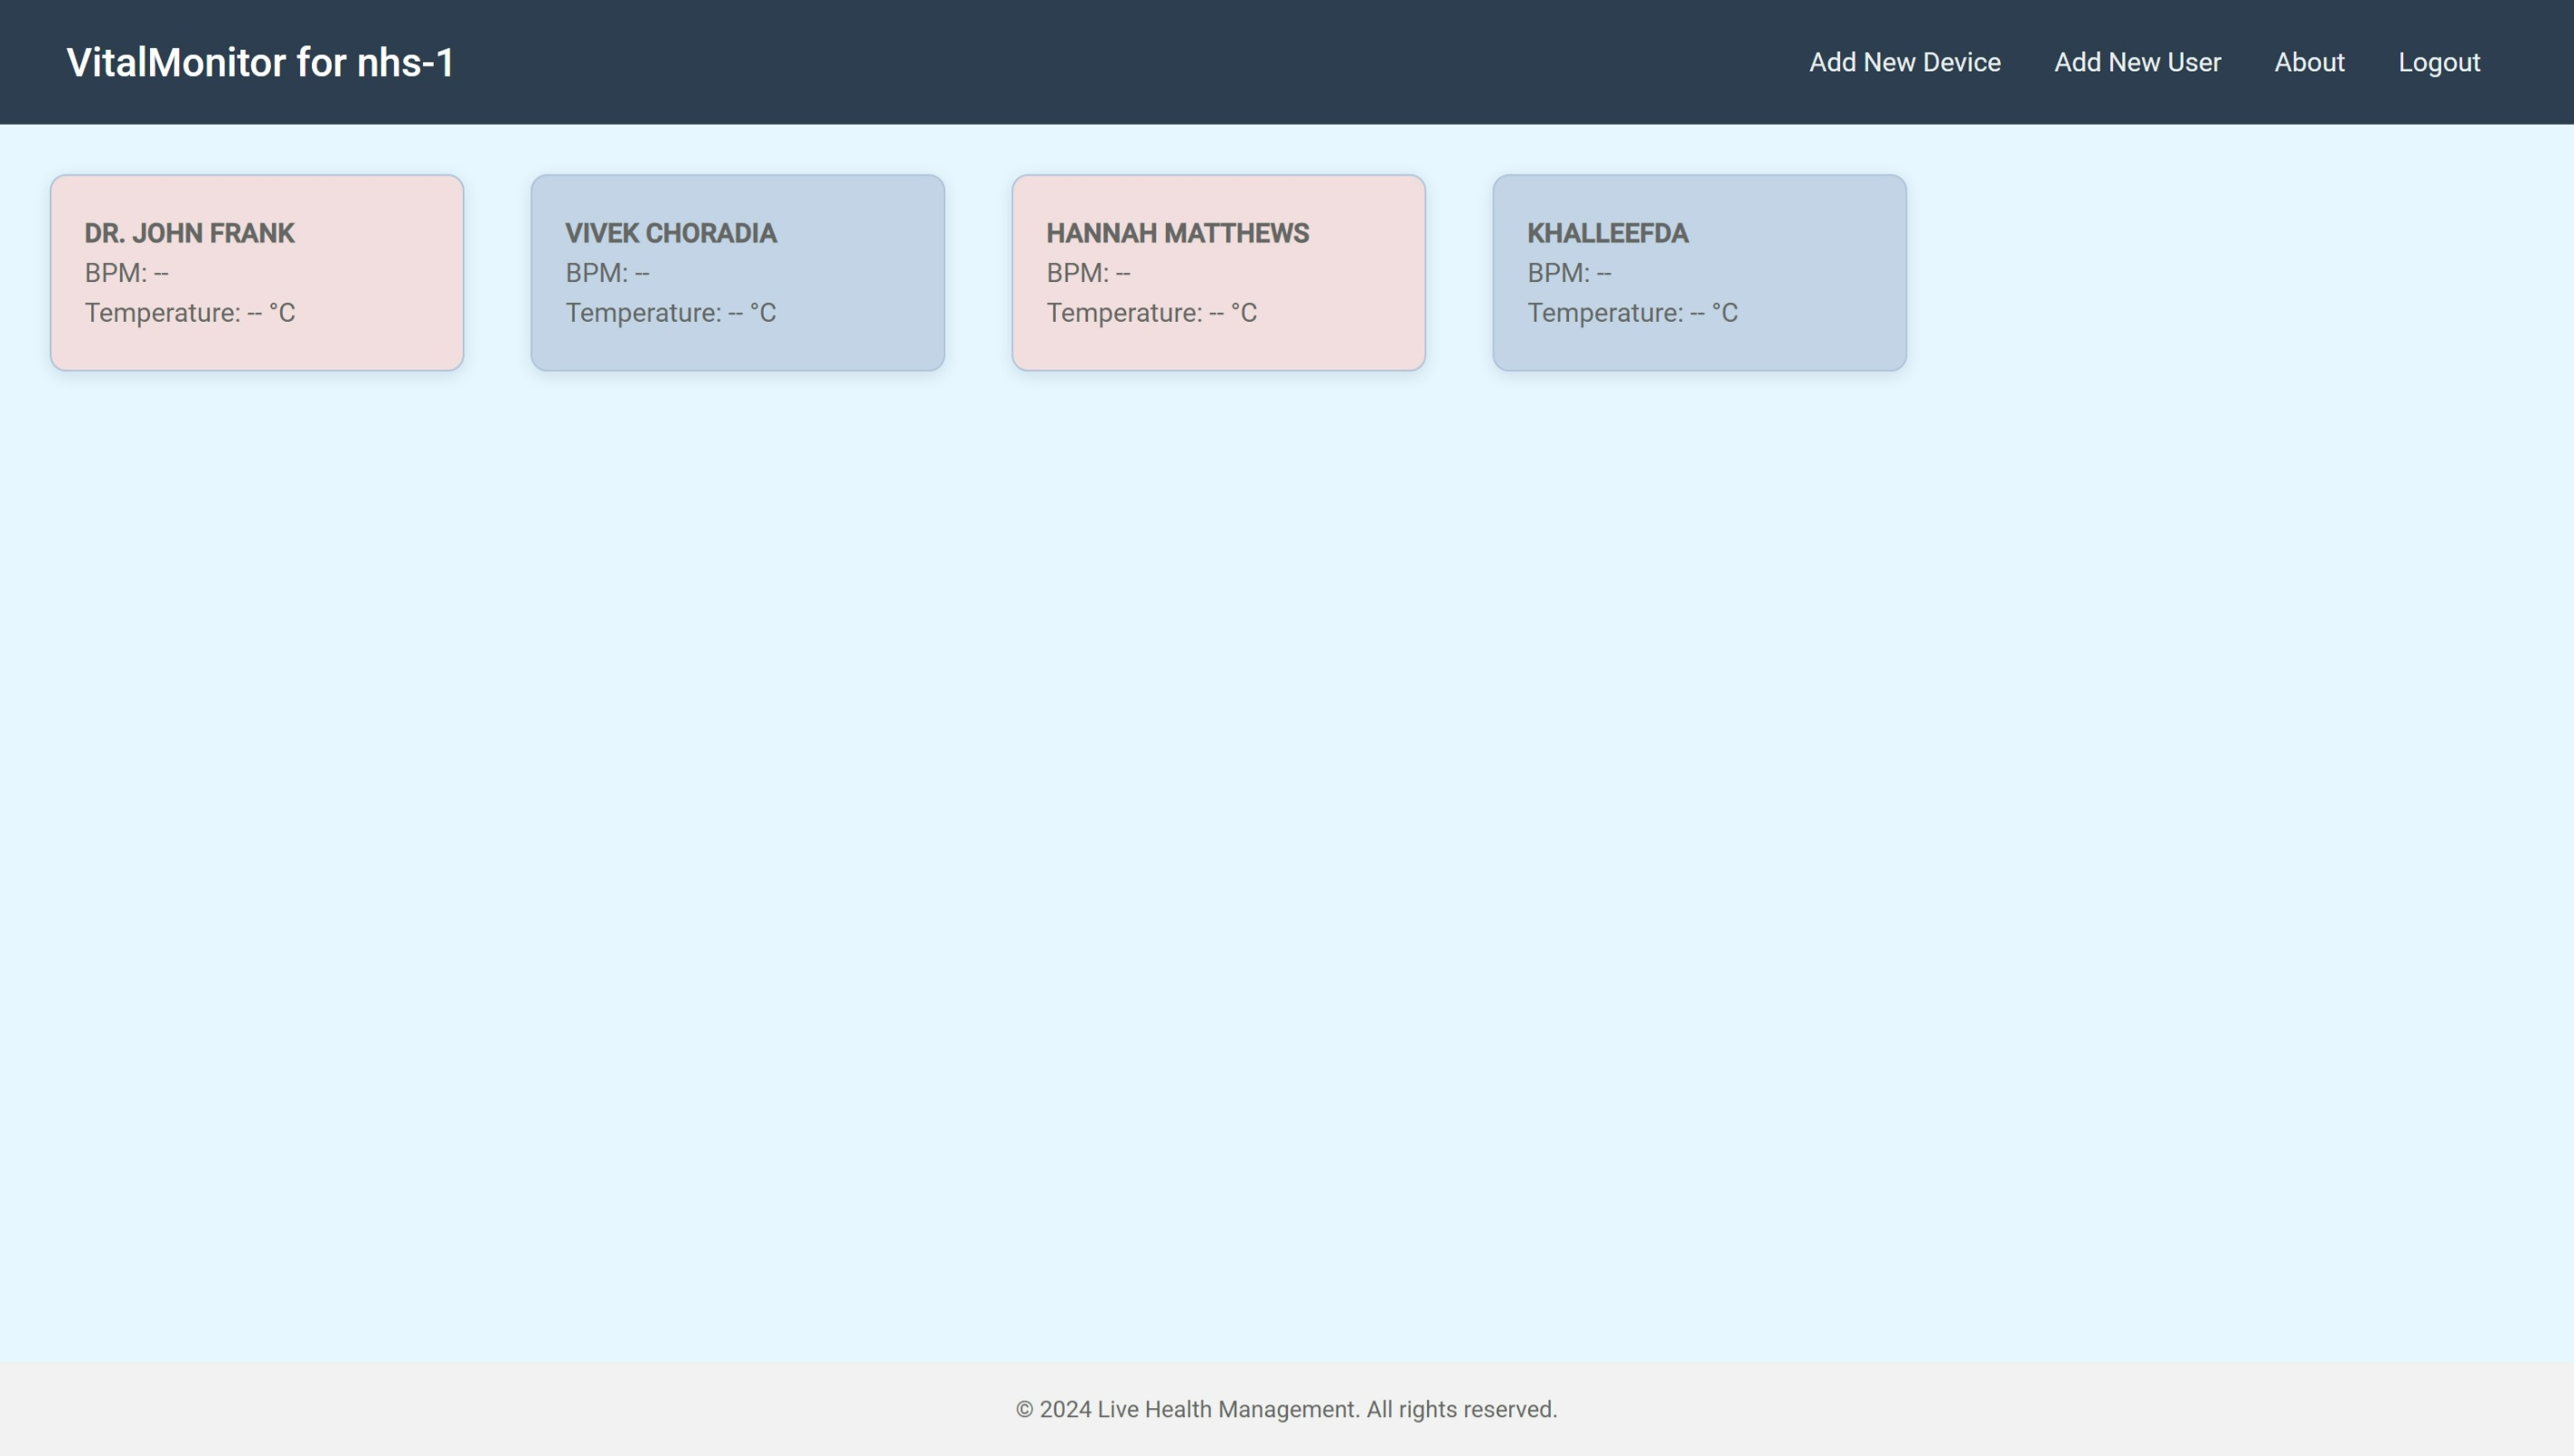
\includegraphics[width=1\linewidth]{images/dashboard-5.jpeg}
    \caption{Home Page}
    \label{fig:home-page}
\end{figure}

\begin{figure}[h!]
    \centering
    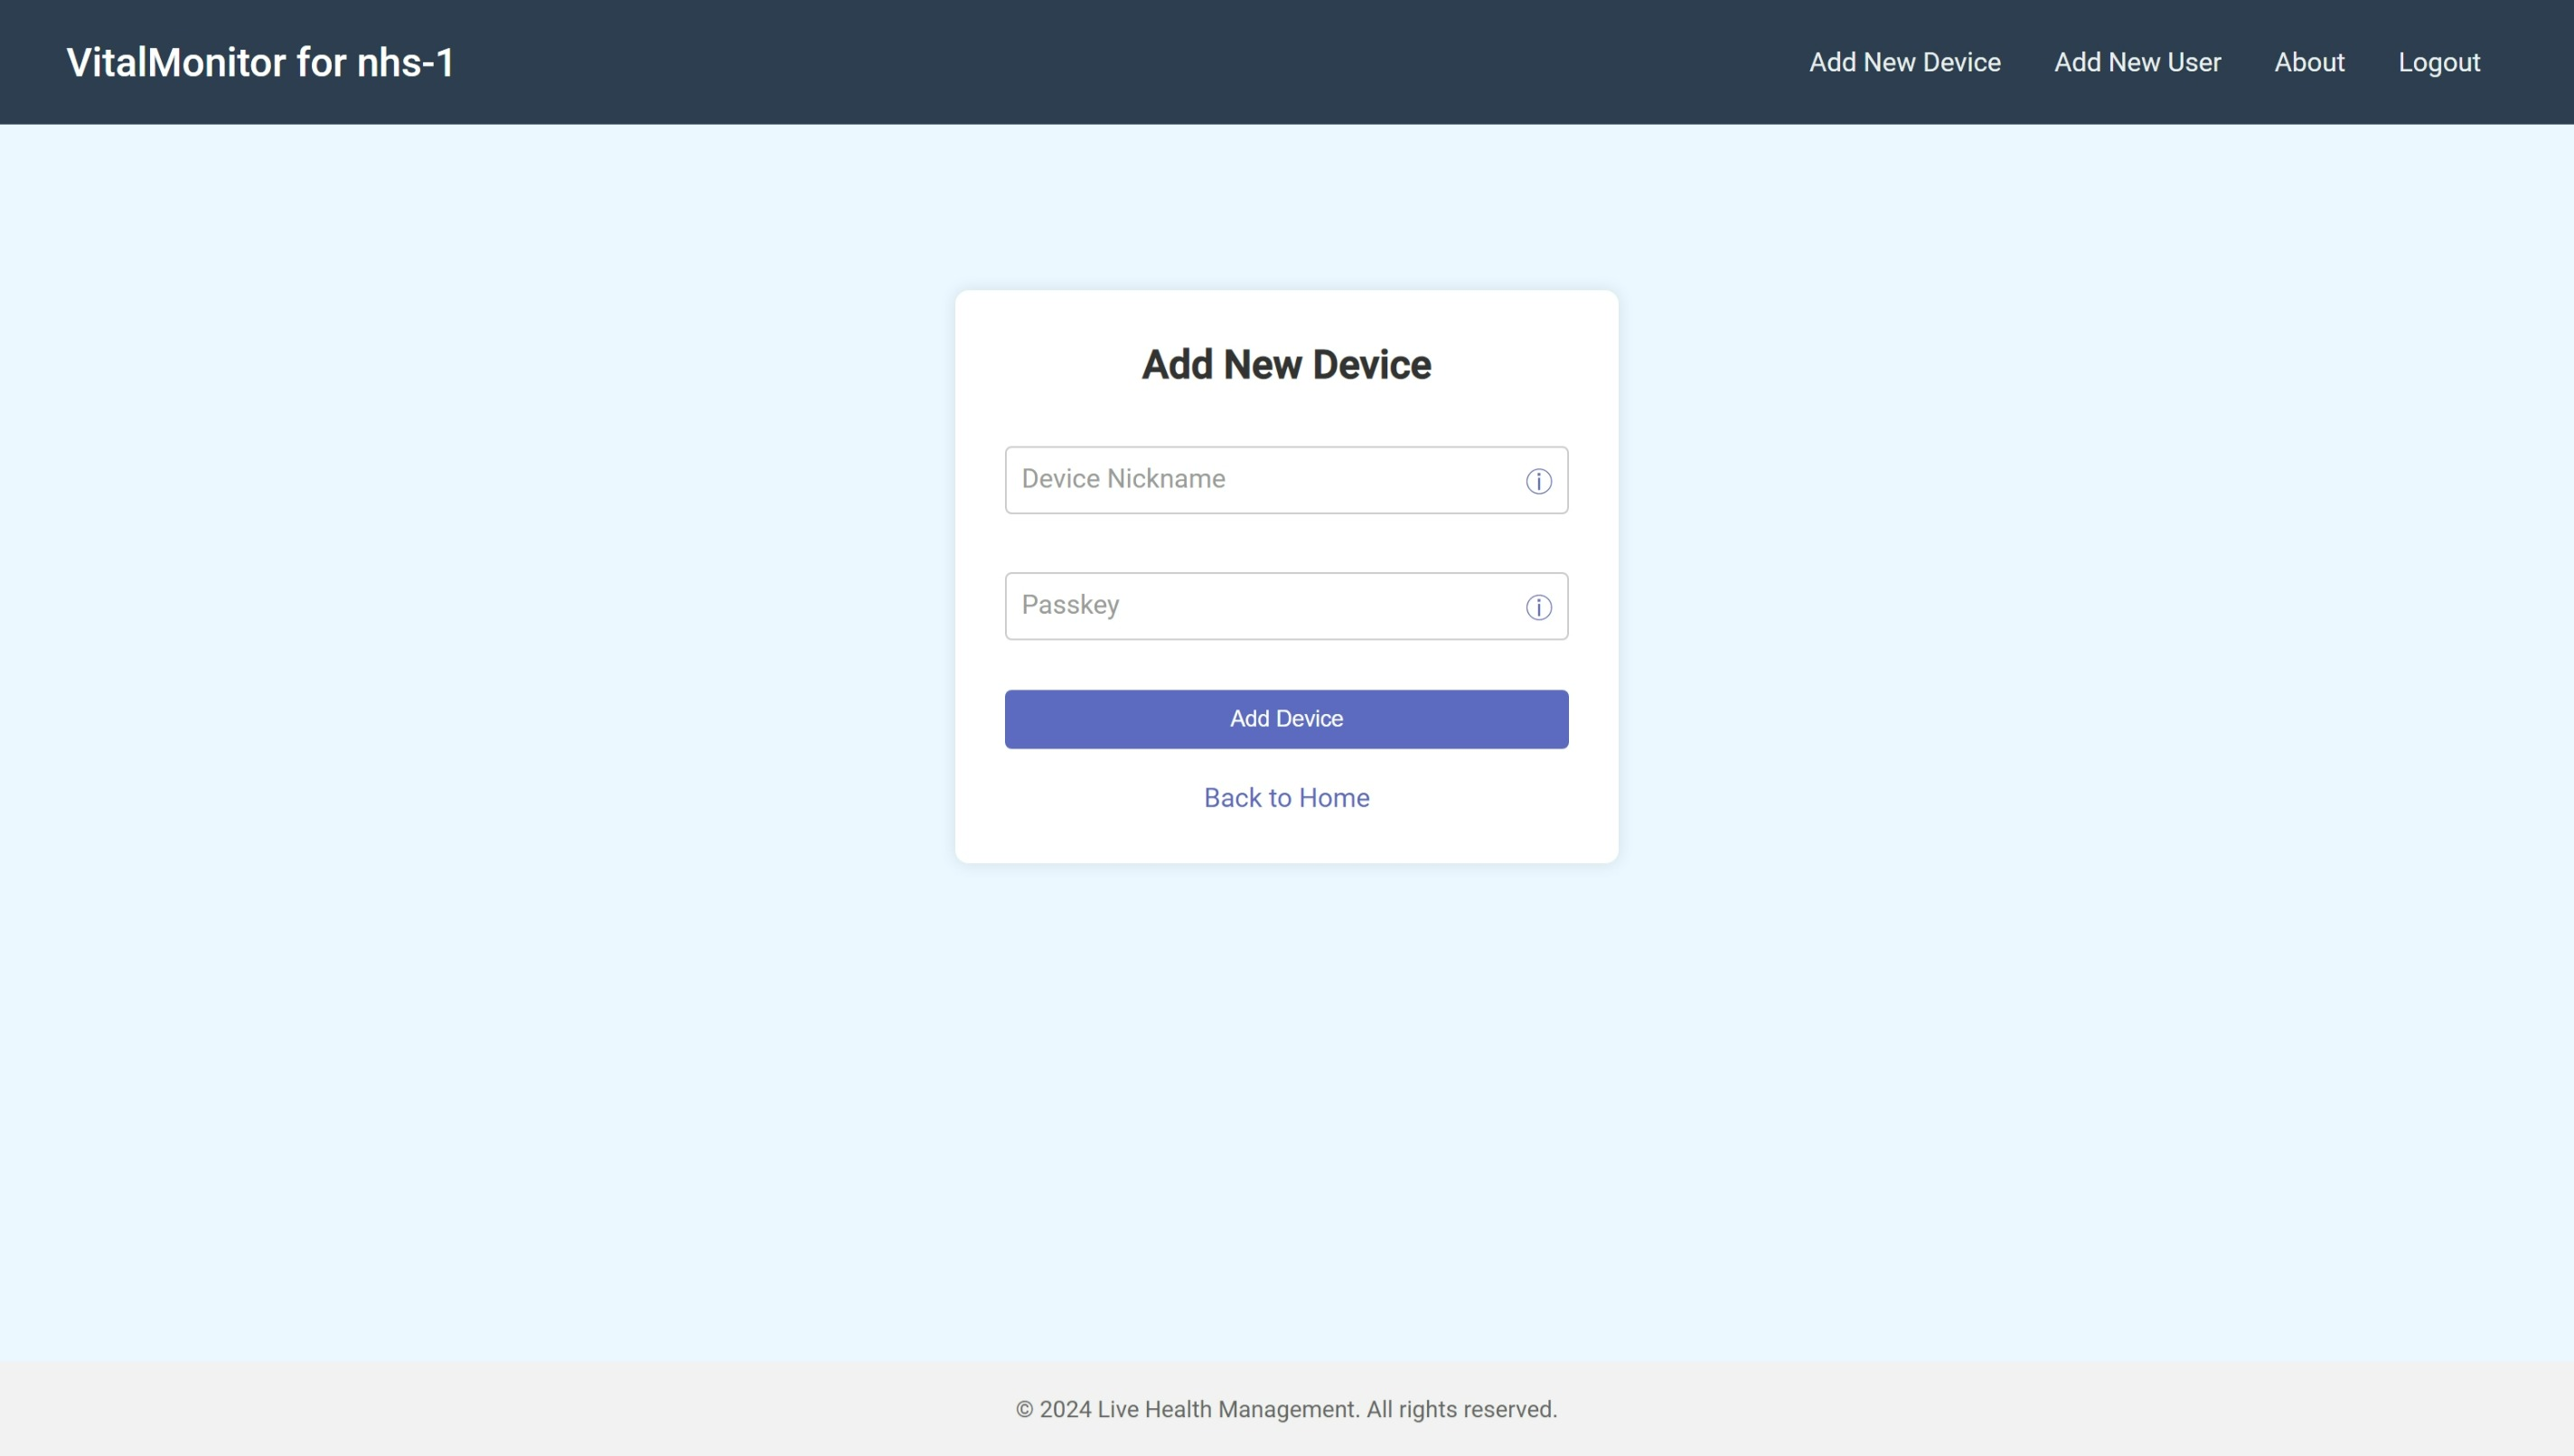
\includegraphics[width=1\linewidth]{images/dashboard-4.jpeg}
    \caption{Add New Device Page}
    \label{fig:device-page}
\end{figure}

\begin{figure}[h!]
    \centering
    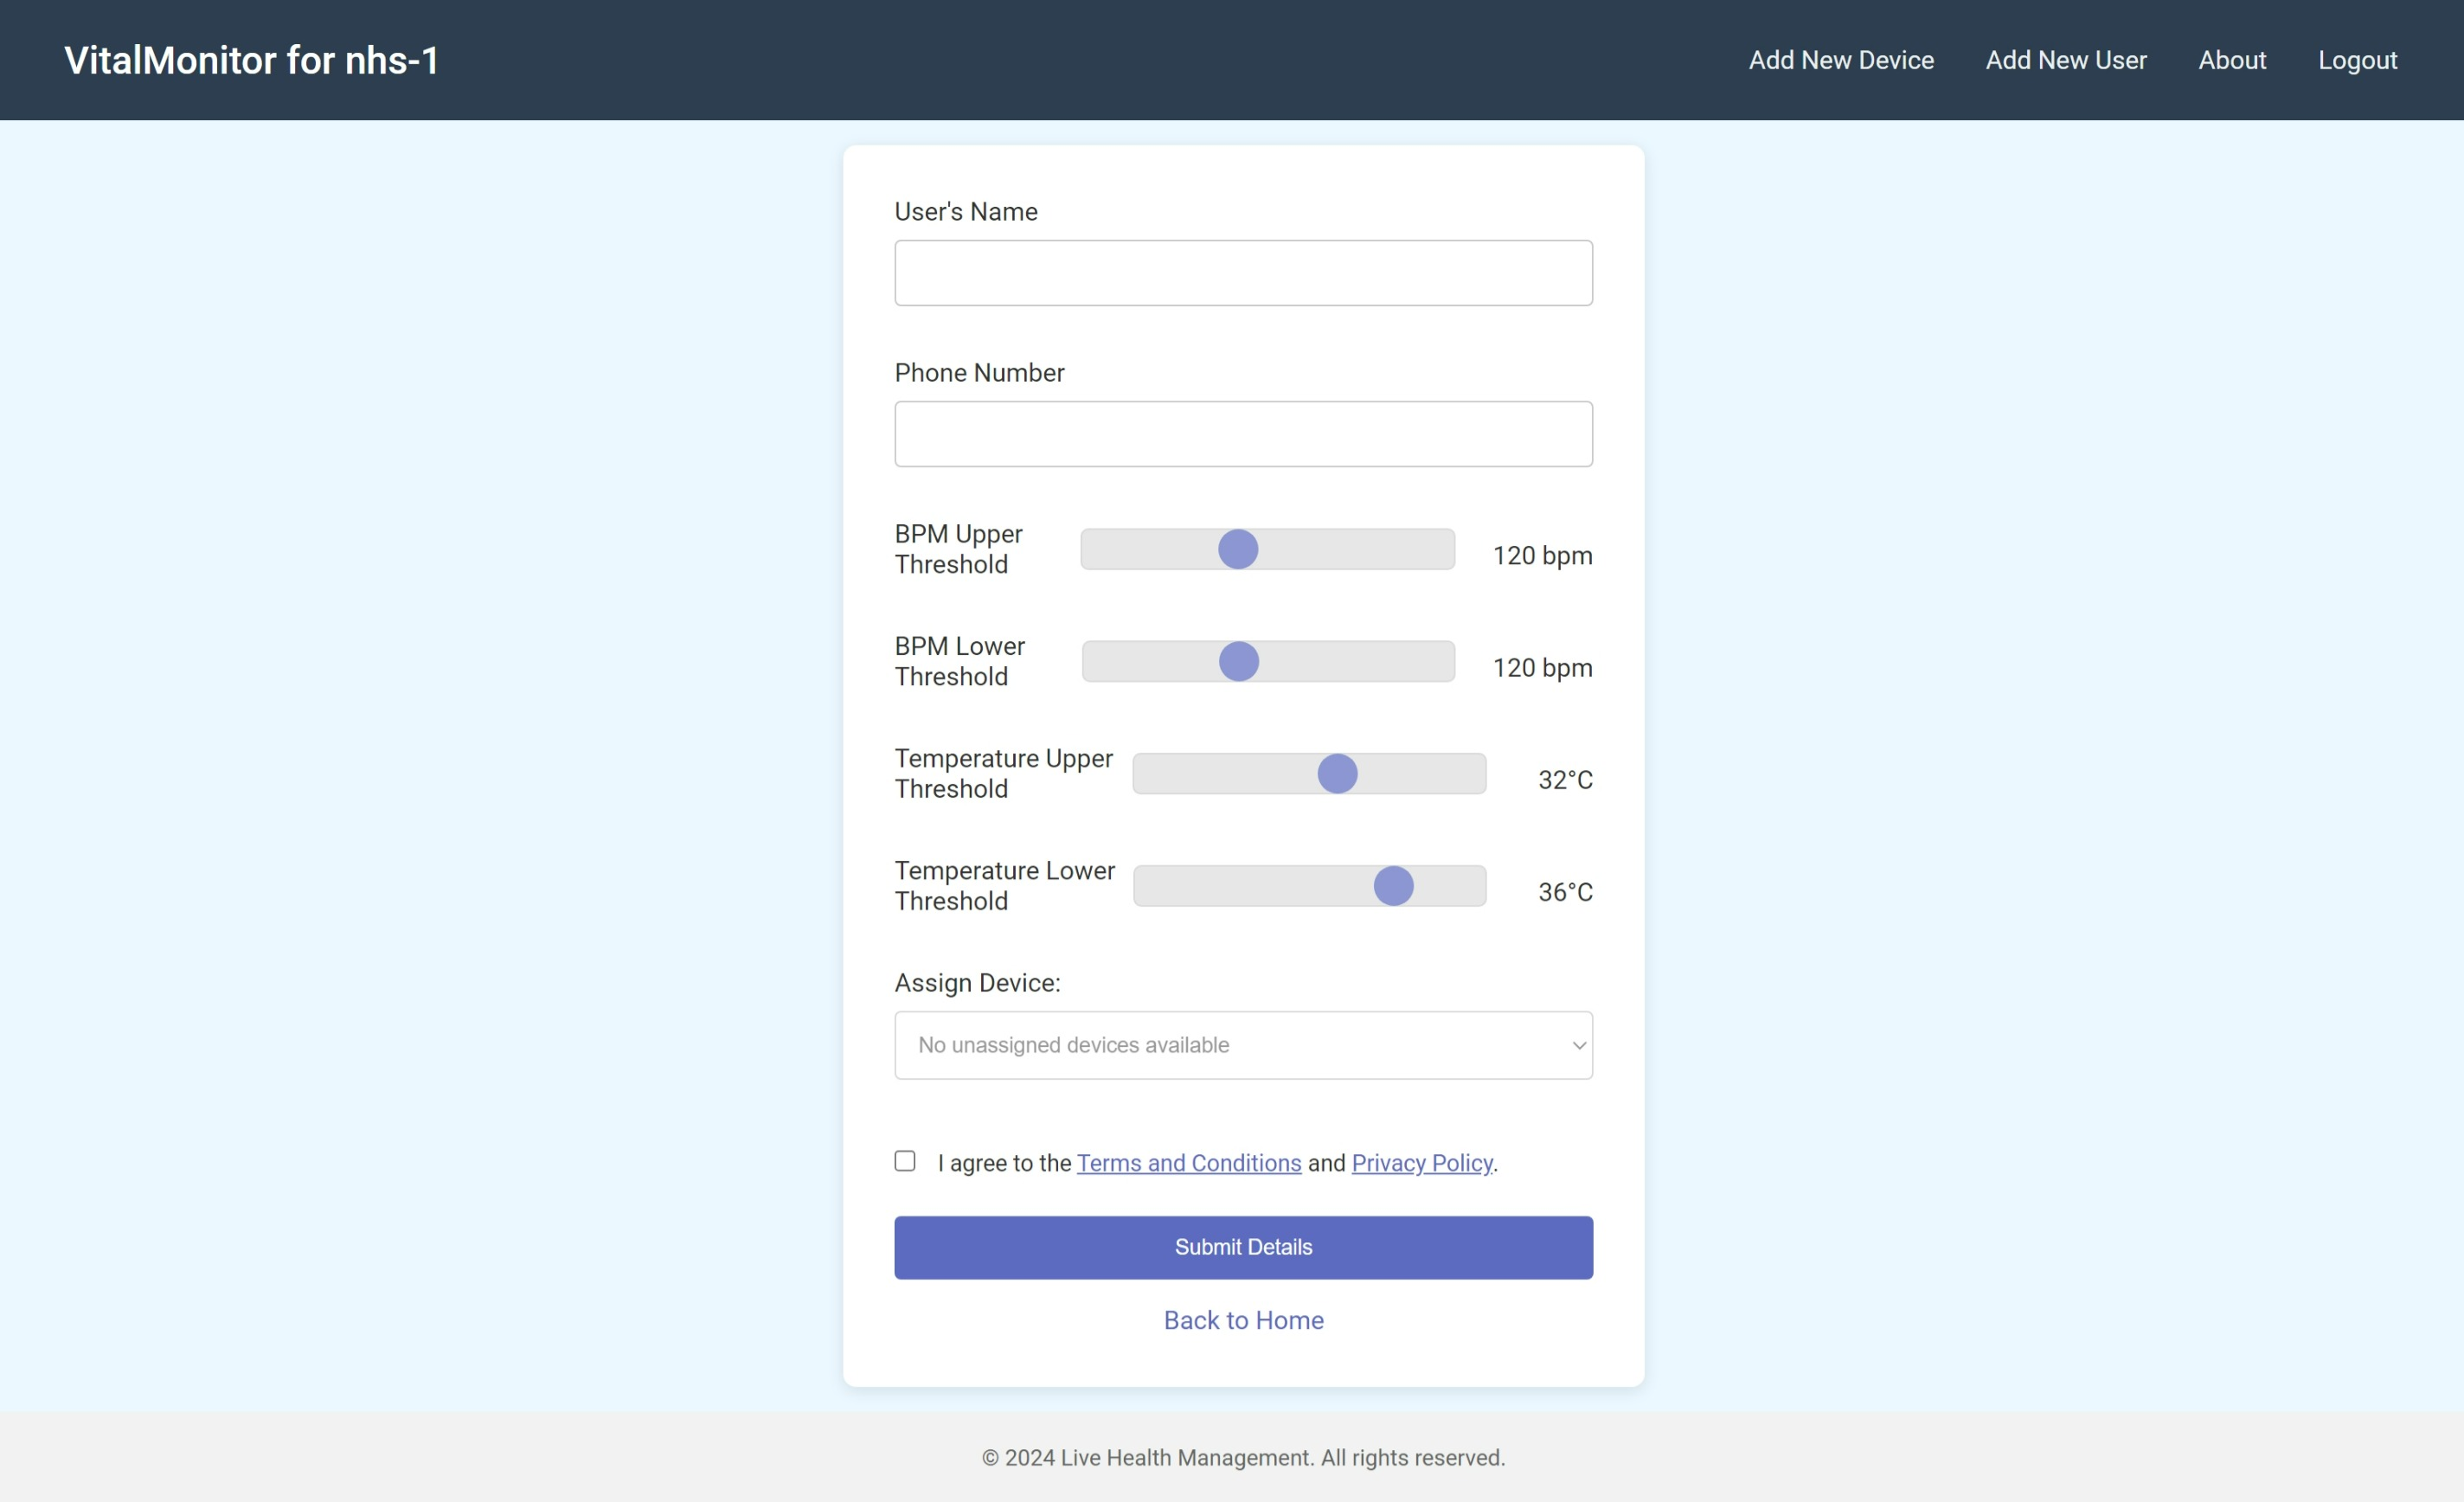
\includegraphics[width=1\linewidth]{images/dashboard-3.jpeg}
    \caption{Add New User Page}
    \label{fig:new-user-page}
\end{figure}

\begin{figure}[h!]
    \centering
    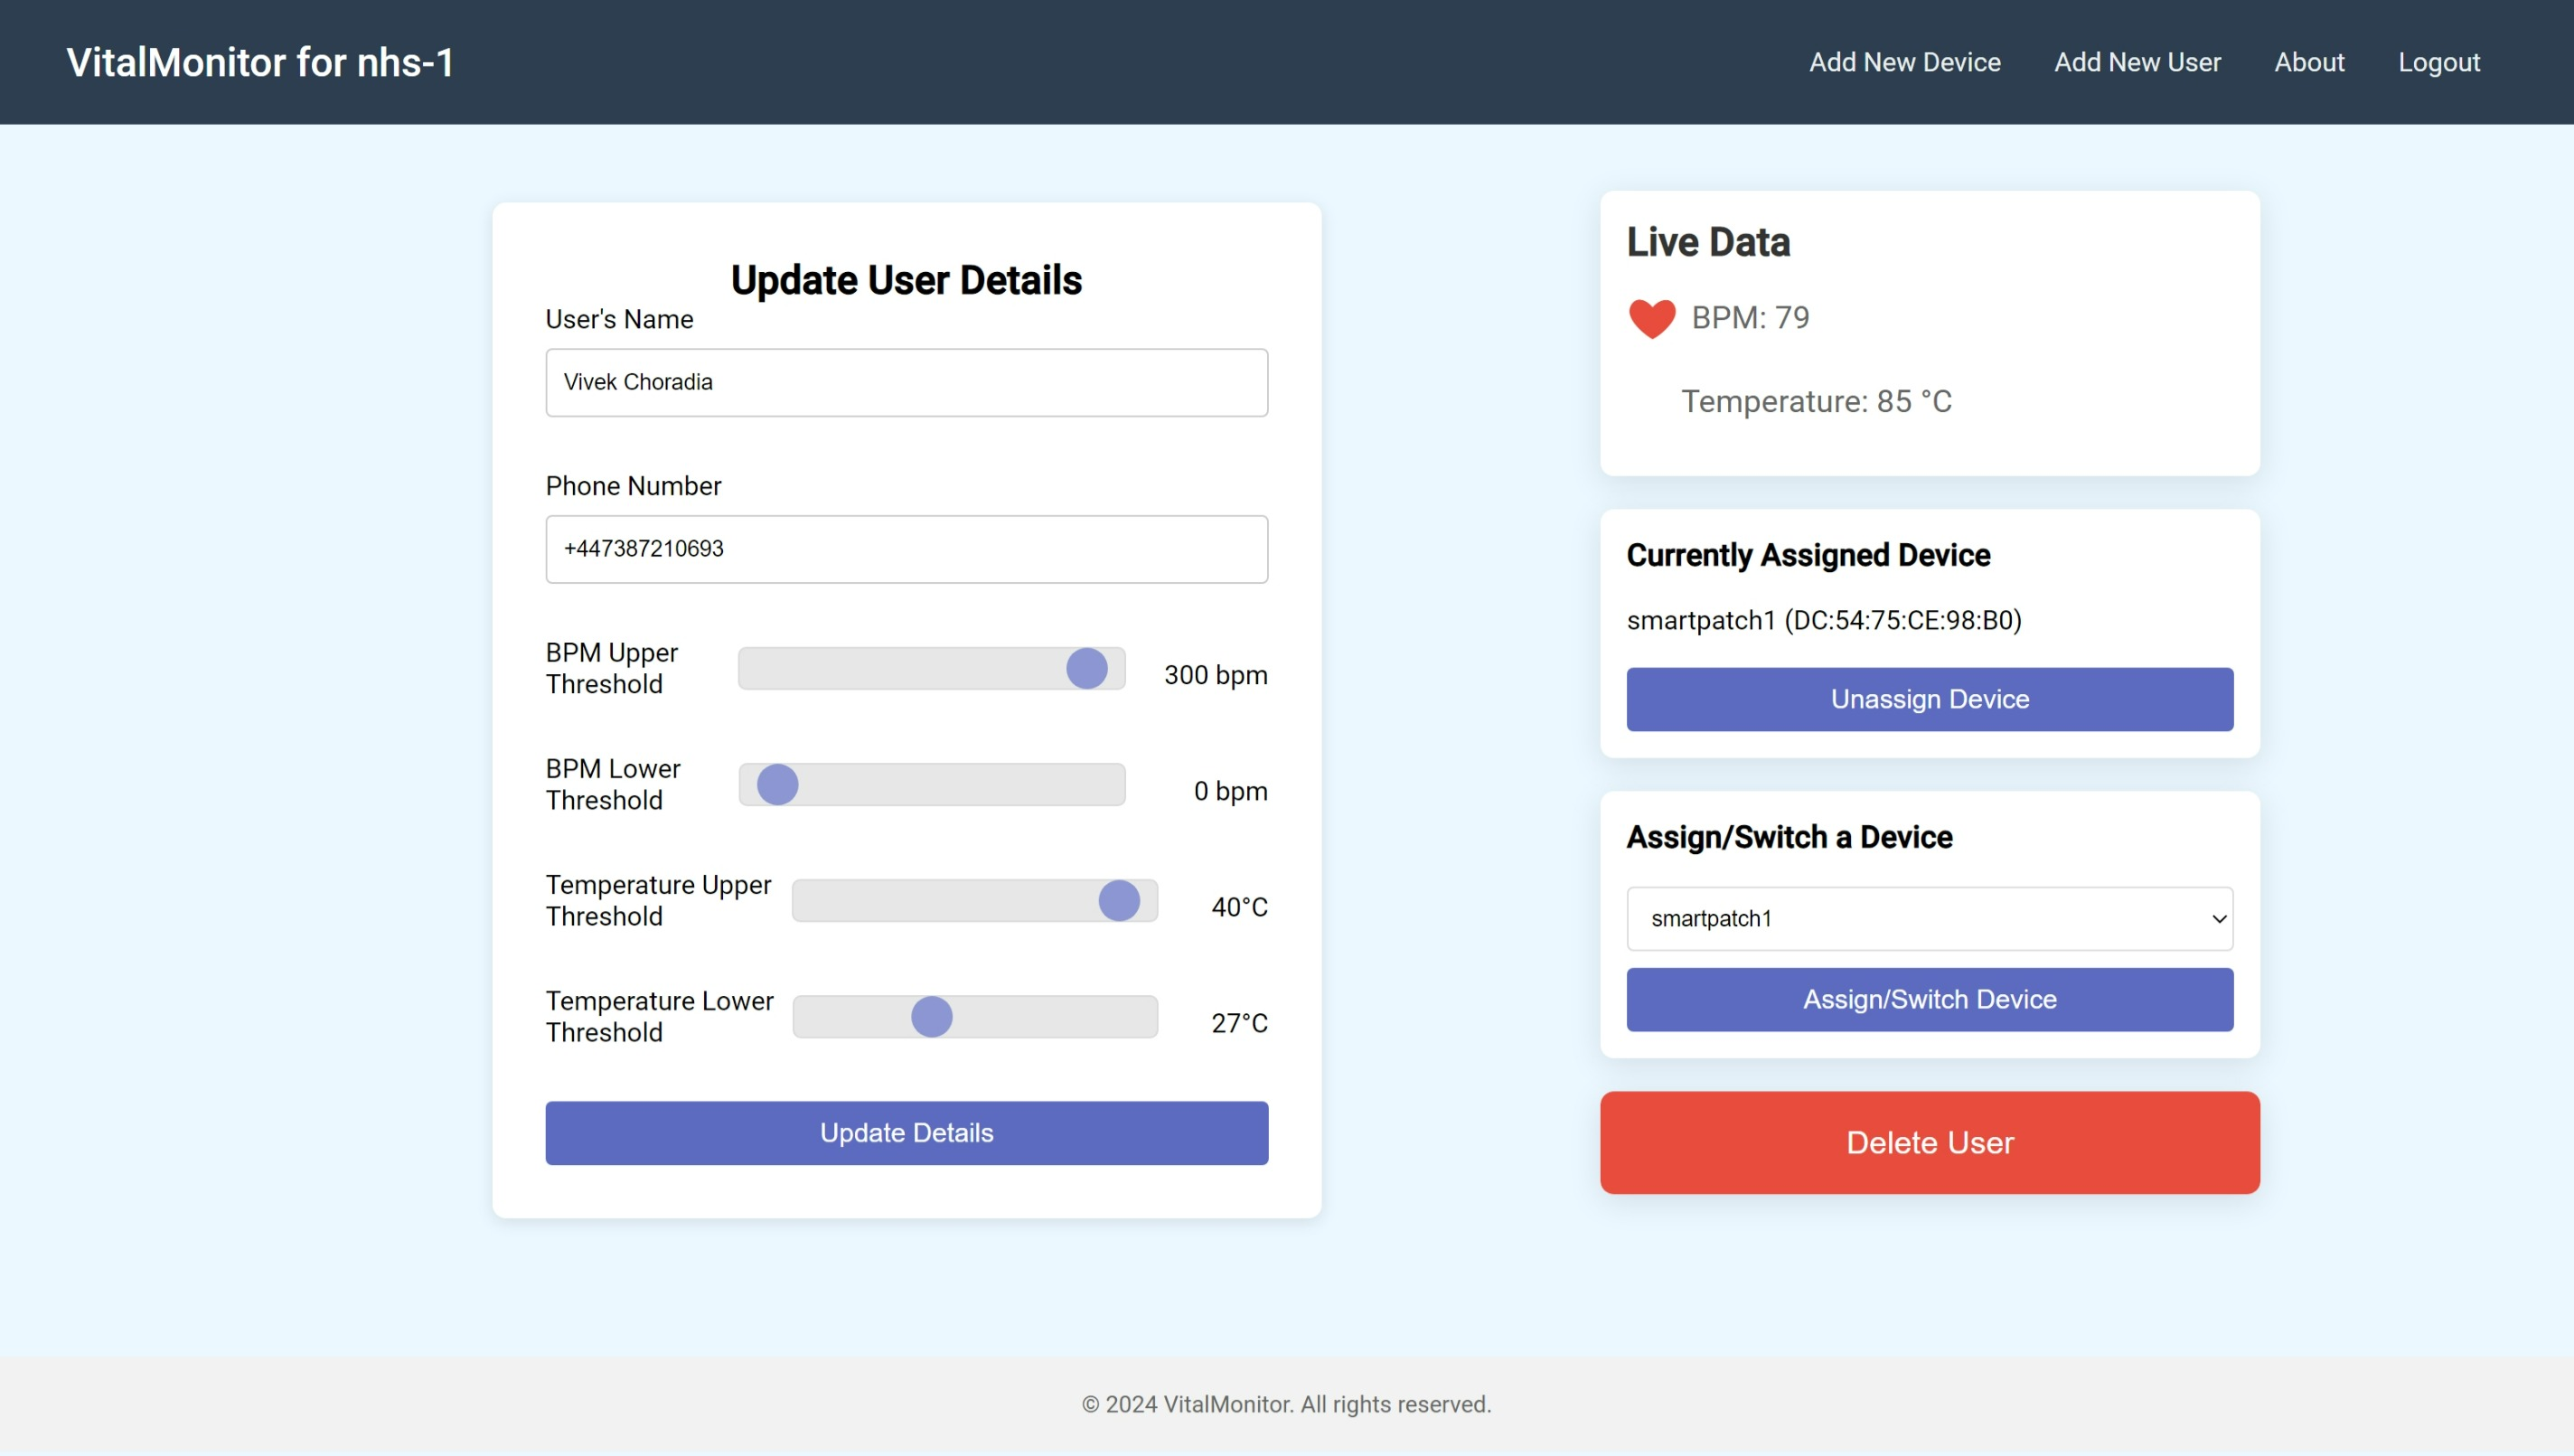
\includegraphics[width=1\linewidth]{images/dashboard-1.jpeg}
    \caption{User Page}
    \label{fig:user-page}
\end{figure}

\begin{figure}[h!]
    \centering
    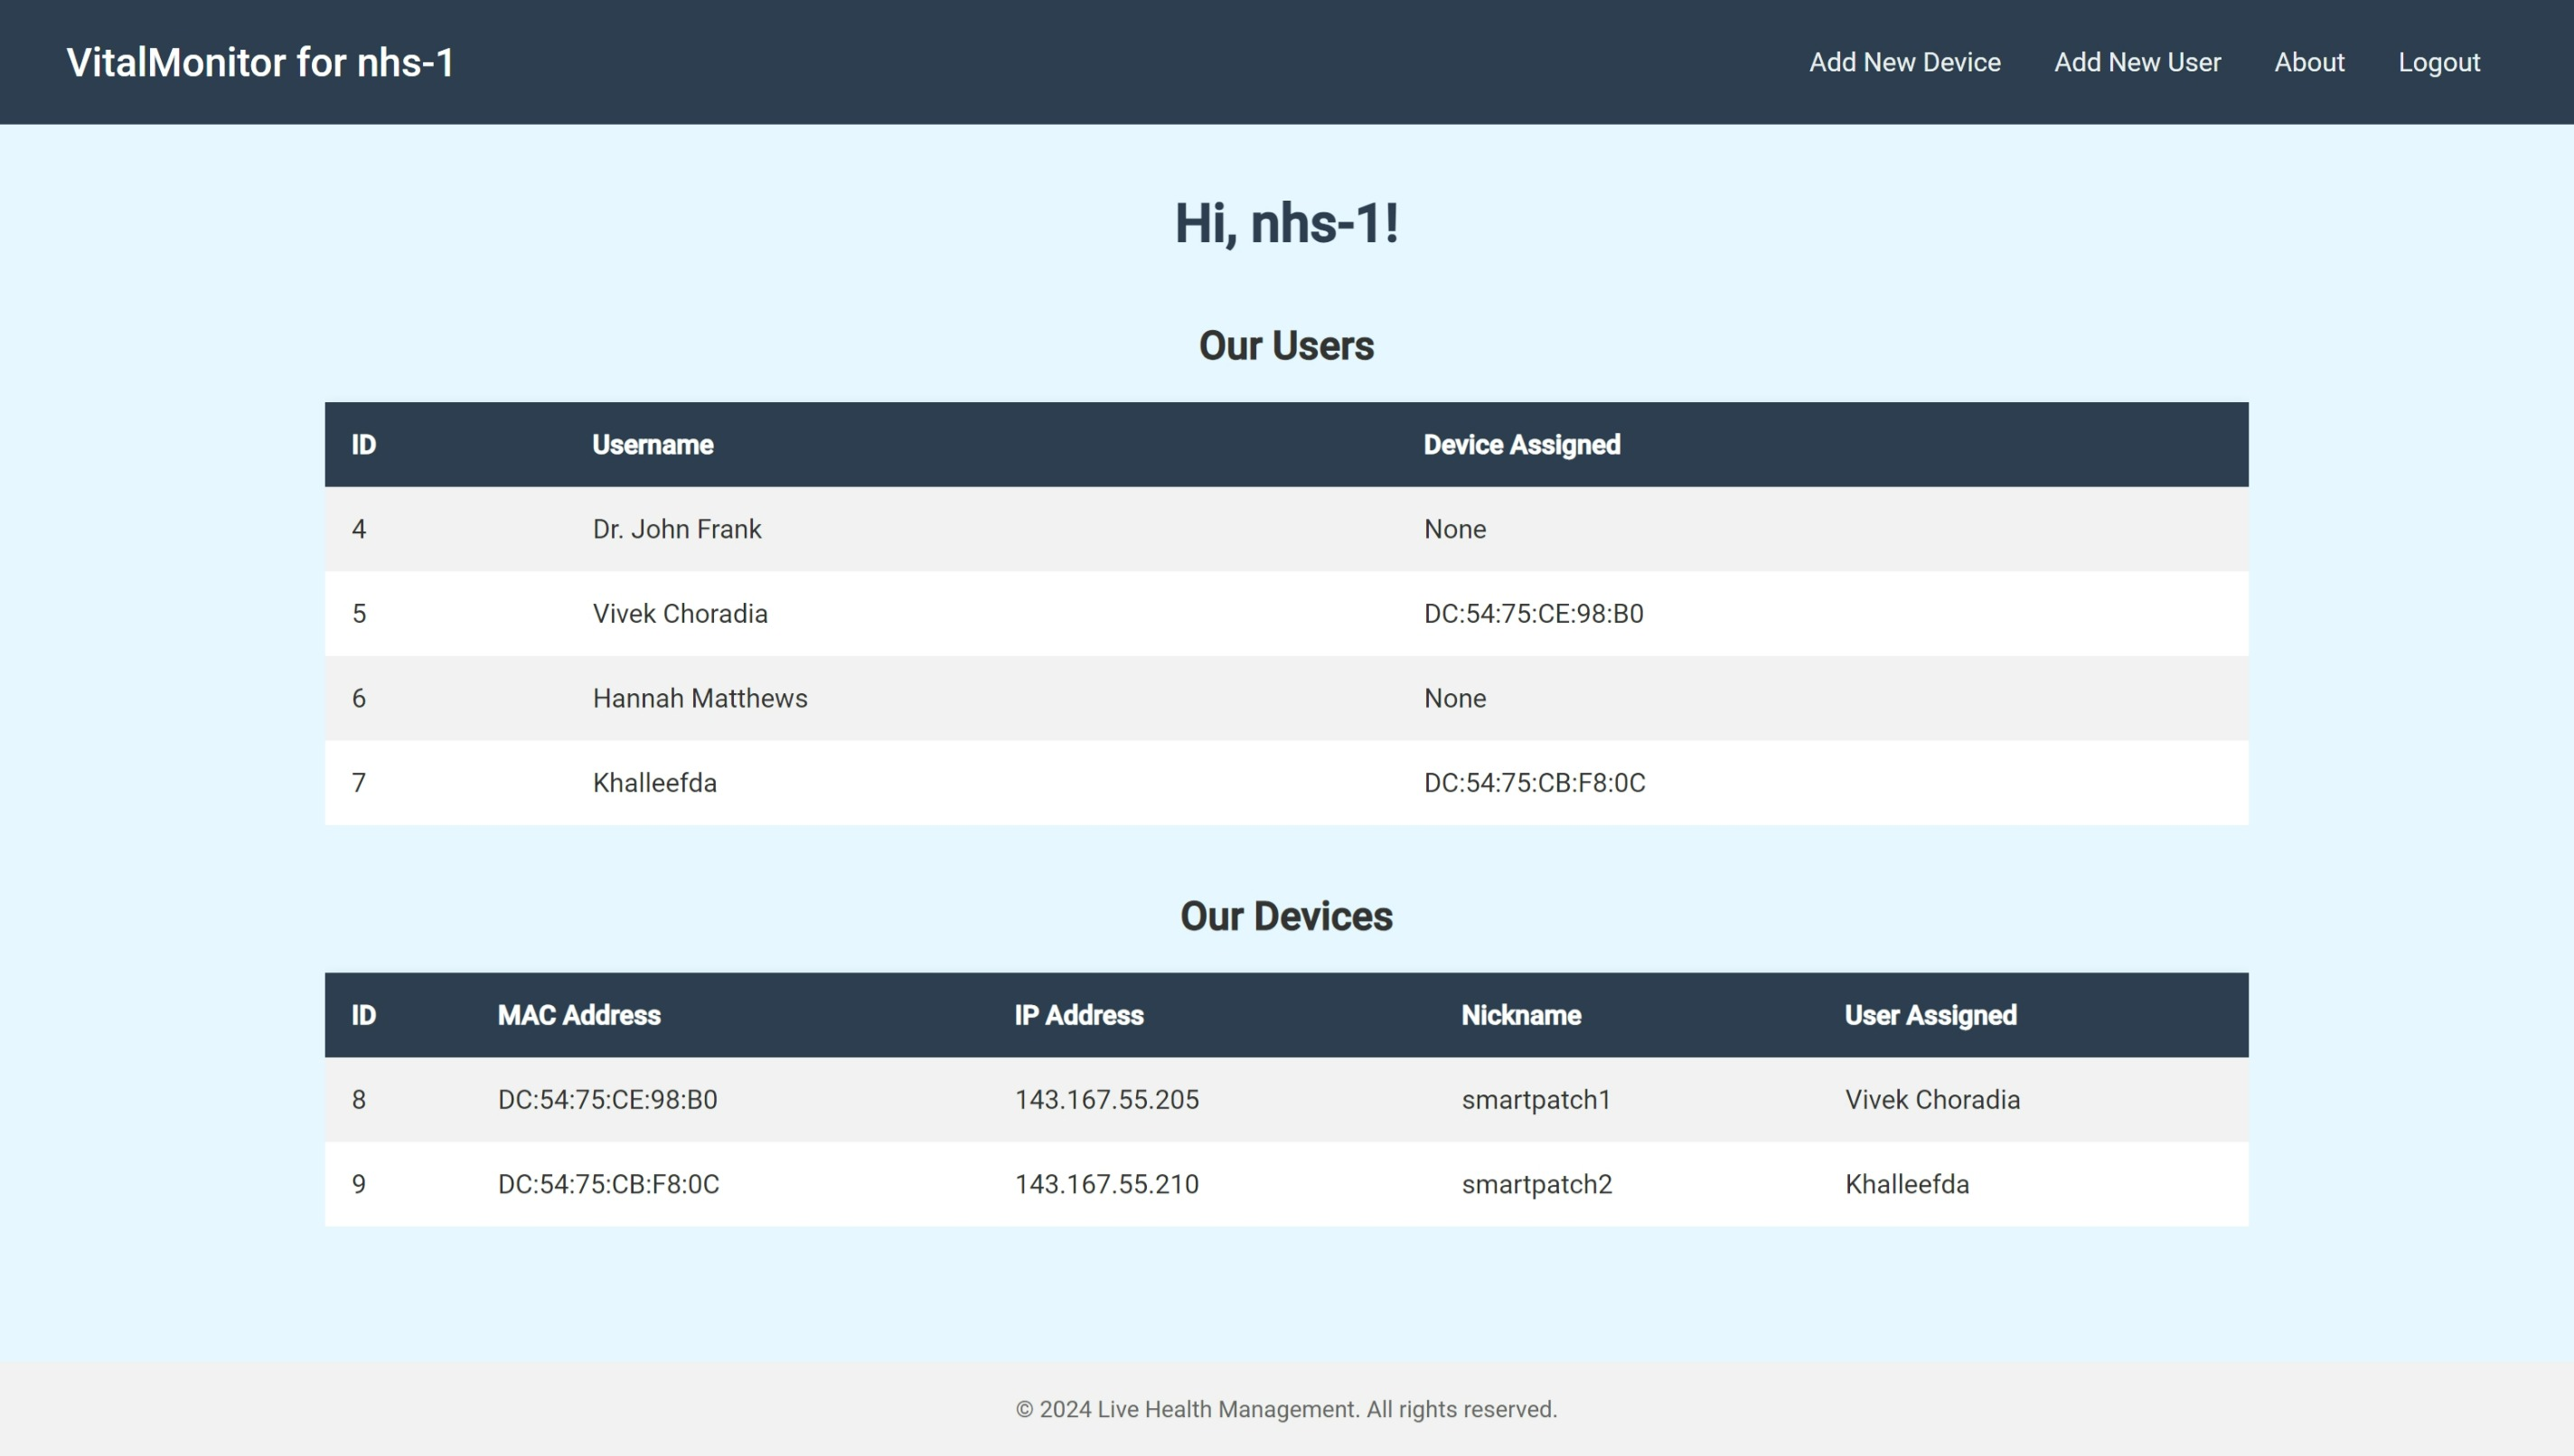
\includegraphics[width=1\linewidth]{images/dashboard-2.jpeg}
    \caption{About Page}
    \label{fig:about-page}
\end{figure}

\clearpage
\noindent Lastly, Privacy policy (refer to Appendix \ref{app:privacy-policy}) and Terms and Conditions (refer to Appendix \ref{app:tnc}) documents were made. Admin using this dashboard, would have to agree to these documents every time they add a new user. This would force admins to ask for permissions of the user using the device that they agree with how they their data is used and they know their rights. 


\section{Testing}
The Testing section details the comprehensive strategies and methodologies used to validate the functionality and reliability of VitalMonitor. This encompasses a range of testing techniques from automated unit and integration tests to manual testing, ensuring the system meets all specified requirements.

\subsection {Acceptance Testing}
Acceptance Testing is important in verifying the system against defined user stories and ensuring that the VitalMonitor functions as intended for end-users. This form of testing is essential for confirming that the system not only functions technically but also fulfills the practical needs of its users. This ensures that the product is ready for deployment and actual use. Each user story is rigorously tested with clear criteria that determine whether the feature is implemented satisfactorily. These tests can be found in the Table \ref{tab:longtable} below.


\begin{longtable}{|c|p{4cm}|p{5cm}|c|}
\caption{User Stories for VitalMonitor Dashboard Implementation} \label{tab:longtable} \\
\hline
\textbf{User Role} & \textbf{Story} & \textbf{Acceptance Criteria} & \textbf{Status} \\ 
\hline
\endfirsthead

\multicolumn{4}{c}%
{{\bfseries Table \thetable\ Continued from previous page}} \\
\hline
\textbf{User Role} & \textbf{Story} & \textbf{Acceptance Criteria} & \textbf{Status} \\
\hline
\endhead

\hline
\multicolumn{4}{|r|}{{Continued on next page}} \\ \hline
\endfoot

\hline
\endlastfoot

Admin & I want to register my organization. & 1. Admin fills and submits a form with organization details. \newline 2. System confirms registration.  & Implemented \\ 
\hline
Admin & I want to log in to the dashboard. & 1. Admin enters credentials. \newline 2. System authenticates and grants access. \newline 3. Error messages are displayed for failures. & Implemented \\
\hline
Admin & I want to add new users. & 1. Admin fills out user form including essential details. \newline 2. Optionally assigns a device. \newline 3. Privacy policy agreement is required for submission. & Implemented \\
\hline
Admin & I want to add new devices. & 1. Admin enters device details. \newline 2. System validates and registers the device. \newline 3. Admin receives confirmation. & Implemented \\
\hline
Admin & I want to manage user-device assignments. & 1. Admin can assign, unassign, or switch devices through user profiles. \newline 2. Updates are immediate and visible. & Implemented \\
\hline
Admin & I want to monitor vital signs in real-time. & 1. Live vital data displayed on user cards. \newline 2. Detailed view available upon clicking a card. \newline 3. Data streams live.  & Implemented \\
\hline
Admin & I want to securely log out. & 1. Admin clicks logout in Navbar. \newline 2. Redirected to login page. \newline 3. Session is cleared.  & Implemented \\
\hline
Admin & I want to view a summary of users and devices. & 1. Admin accesses About Page from Navbar. \newline 2. Page lists all resources. \newline 3. Options for data reporting and exporting available. & Implemented \\ \hline
User & I want to wear the device comfortably on my ear (Future Implementation). & 1. The device is lightweight and designed to fit securely on the ear. \newline 2. Users report comfort and lack of interference with daily activities. & Not Started \\
\hline
User & I want to easily activate the Smart Patch by pressing a button. & 1. The device has a single button for activation. \newline 2. Pressing the button turns on the device and starts data transmission, indicated by a red light. & Implemented \\
\hline
User & I want to press the button again to stop sending data. & 1. Pressing the button a second time turns off the device and stops data transmission, indicated by the red light turning off. \newline 2. Data stops being published immediately. & Implemented \\
\hline
User & I want the device to continuously measure my heart rate and body temperature while activated. & 1. The device measures heart rate and body temperature in real-time. \newline 2. Data is sent to the system at regular intervals without delay while the device is on. & Implemented \\
\hline
\end{longtable}


\subsection{System and Integration Testing}

System and Integration Testing play a crucial role in ensuring the reliability and functionality of VitalMonitor's API endpoints. These tests aim to validate the behavior of the system as a whole and the interactions between its various components. VitalMonitor employs a testing approach, primarily using curl commands to interact with API endpoints. This approach allows for thorough validation of each endpoint's functionality and behavior in different scenarios.  \\

\noindent Various testing scenarios are covered to ensure the robustness of VitalMonitor's API endpoints:
\begin{enumerate}
    \item \textbf{Endpoint Functionality}: Each API endpoint is tested to verify its functionality, including creating, updating, retrieving, and deleting resources such as organizations, users, and devices.
    \item \textbf{Data Validation}: Input data is tested for validity and completeness, ensuring that endpoints handle both valid and invalid data gracefully. This includes testing edge cases and boundary conditions.
    \item \textbf{Error Handling}: Error scenarios are tested to validate the system's behavior when encountering errors, such as missing parameters, unauthorized access, or internal server errors. The responses are examined to ensure they provide meaningful error messages and appropriate status codes.
    \item \textbf{Integration Testing}: Endpoints that interact with external systems, such as devices or external APIs, are thoroughly tested to ensure seamless integration and proper data exchange.
\end{enumerate}

Curl commands are utilized to perform these testings of VitalMonitor's API endpoints. These commands are executed from the command line interface and simulate HTTP requests to interact with the system. One example of such command and the response received is shown in Figure \ref{fig:curl-command}:

\begin{figure}[h!]
    \centering
    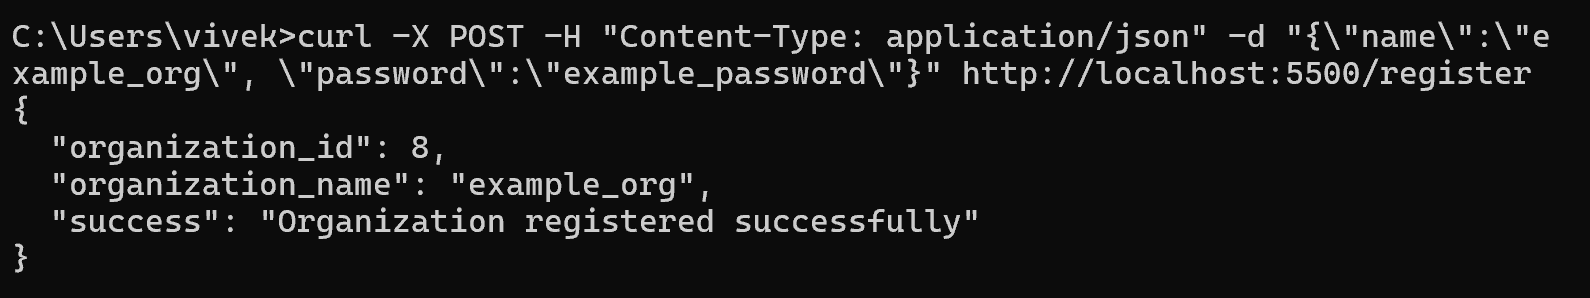
\includegraphics[width=1\linewidth]{images/curl-command.png}
    \caption{CURL Command to test whether adding organization }
    \label{fig:curl-command}
\end{figure}


\subsection{Unit Testing}
Unit testing for both the middleware and the web dashboard was rigorously conducted to ensure robustness and functionality across all components. These tests were implemented using the \textit{pytest} framework and the flask-testing library, supplemented by additional tools such as \textit{contextlib}, \textit{unittest.patch}, \textit{unittest.mock}, \textit{sqlalchemy.exc}, and \textit{requests.exceptions}. This robust toolkit facilitated a comprehensive testing approach, encompassing both functional correctness and error handling capabilities. \\

\noindent To avoid impacting the development database, a dedicated local SQLite database was provisioned for the duration of the testing phase. This temporary database was programmatically created prior to each test suite and subsequently destroyed upon completion, ensuring a clean slate for each test run and preventing data persistence that could skew test outcomes.\\

\noindent Furthermore, in order to fully simulate API interactions without actual external API calls, mock responses and requests were meticulously crafted. This allowed for controlled testing of API functionalities and error handling without the need for live network conditions, thereby increasing the reliability of the test outcomes. However, certain interactions, such as data exchanges with other subsystems, could not be effectively simulated within this framework. These scenarios were addressed through targeted manual testing to ensure comprehensive coverage.\\

\noindent Coverage analysis was conducted using the \textit{coverage.py} tool, providing insights into the extent of code executed by the tests and highlighting any areas lacking in test coverage. This analysis was crucial in identifying untested paths and informed subsequent test development to ensure a high degree of code coverage.\\

The results of these efforts are as follows: 
\begin{itemize}
    \item The middleware was subjected to 37 unit tests, with the coverage outcomes detailed in Figure \ref{fig:middleware-coverage}.
    \begin{figure}[h!]
    \centering
    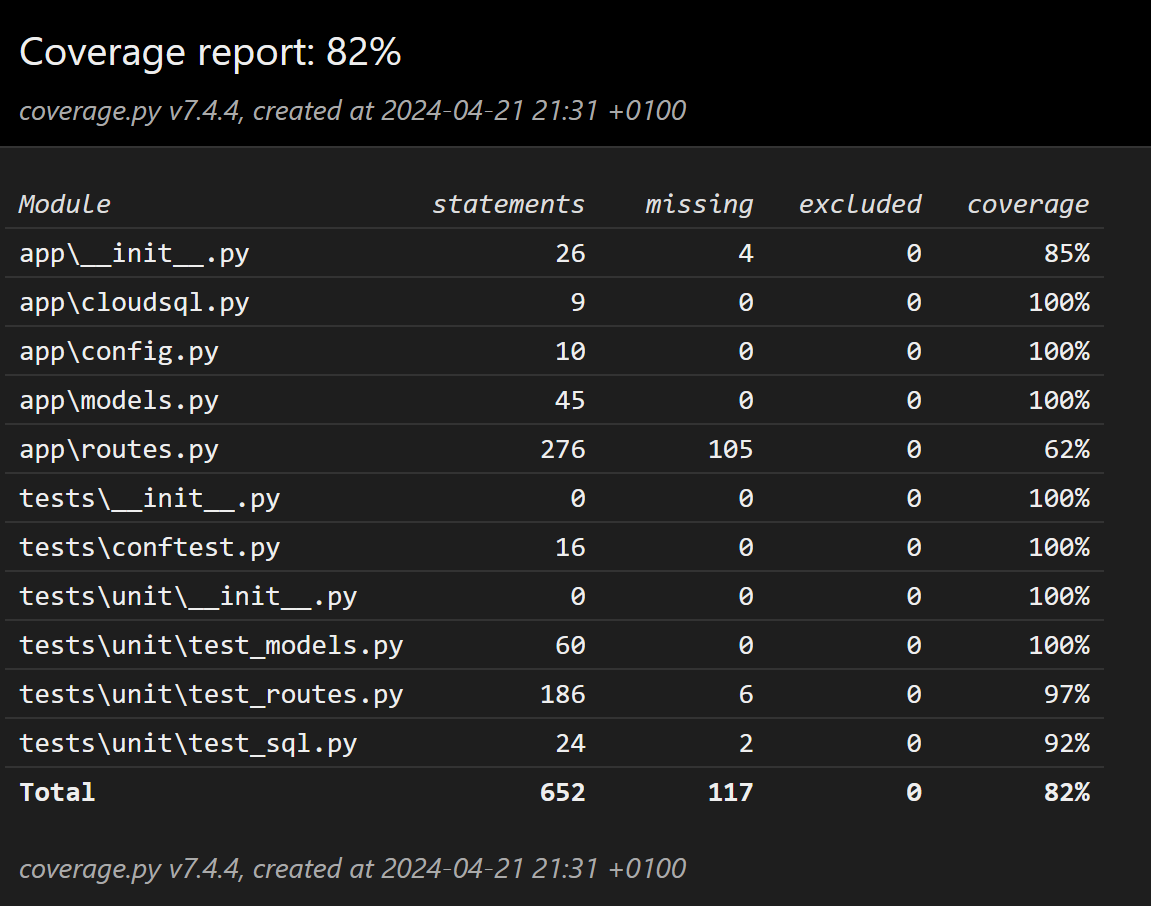
\includegraphics[width=0.7\linewidth]{images/middleware-coverage.png}
    \caption{Middleware Coverage}
    \label{fig:middleware-coverage}
\end{figure}
    \item The web dashboard underwent a series of 27 unit tests, with its respective coverage report depicted in Figure \ref{fig:web-dashboard-coverage}.
    \begin{figure}[h!]
    \centering
    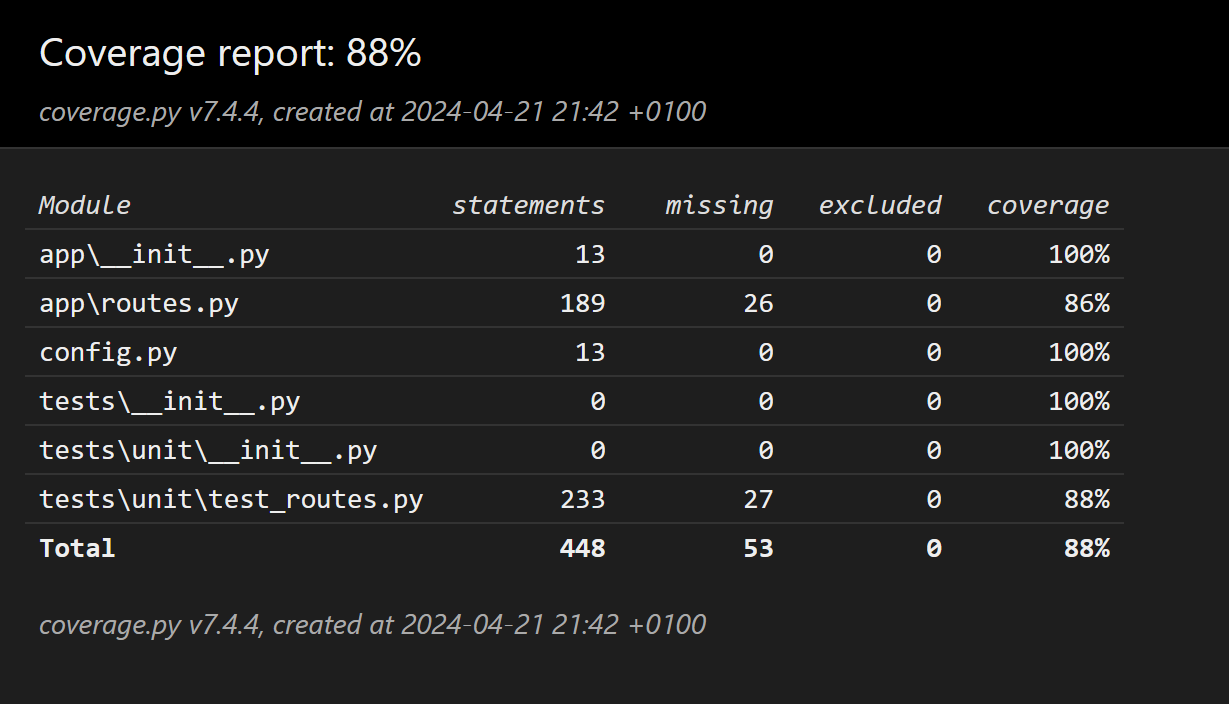
\includegraphics[width=0.7\linewidth]{images/webdashboard-coverage.png}
    \caption{Web Dashboard Coverage}
    \label{fig:web-dashboard-coverage}
\end{figure} 
\end{itemize}



\newpage
\subsection{Manual Testing}

Manual testing was rigorously conducted on both the Web Dashboard and the Smart Patch to ensure comprehensive validation of system functionalities not covered by automated tests. This process is crucial for verifying the integrated operation of all subsystems, offering insights into real-world usability and interaction sequences that automated tests might overlook. \\

\noindent For a structured approach, each test case was assigned a unique Test Case ID, with meticulously detailed test procedures and clearly defined expected results. The outcomes of these tests were diligently recorded, specifying whether each test case passed or failed, thus providing a transparent and accountable testing framework. \\

\noindent The example below illustrates the methodical nature of our manual testing approach:

\begin{longtable}{|c|p{5cm}|p{4cm}|c|}
\caption{Manual Test Cases for Smart Patch Device} \label{tab:manual_tests_device} \\
\hline
\textbf{Test Case ID} & \textbf{Test Details} & \textbf{Expected Results} & \textbf{Pass/Fail} \\
\hline
\endfirsthead

\multicolumn{4}{c}%
{{\bfseries Table \thetable\ Continued from previous page}} \\
\hline
\textbf{Test Case ID} & \textbf{Test Details} & \textbf{Expected Results} & \textbf{Pass/Fail} \\
\hline
\endhead

\hline
\multicolumn{4}{|r|}{{Continued on next page}} \\ \hline
\endfoot

\hline
\endlastfoot

TC-SP01 & Verify activation of the Smart Patch by pressing the button. \newline
- Ensure the device is off. \newline
- Press the activation button. & Device turns on (red light indicator) and starts transmitting data. & Pass \\
\hline
\end{longtable}

A comprehensive list of all manual test cases, along with their respective details and outcomes, is provided in the \textbf{Appendix \ref{app:manual-testing}}. This meticulous documentation facilitates an in-depth understanding of the product’s performance in real-world scenarios and ensures all subsystems function harmoniously together.
